The $\MET$ cut applied in the signal region is $\MET > $ 20 GeV.
Therefore the region $\MET < $ 20 GeV can be taken as a control
region. In the control region, the data, and MC comparison after kinematic fit selection are shown in
Figures~\ref{fig:LowMET_kfitPlot1}, \ref{fig:LowMET_kfitPlot2}, \ref{fig:LowMET_kfitPlot3}, \ref{fig:LowMET_mjjInc}, 
\ref{fig:LowMET_mjjCTagL}, \ref{fig:LowMET_mjjCTagEx}. In these plots, the MC QCD
events have been used which are concentrated in few bins only. 
Overall, there is a good agreement between data and MC in the control region.

%After KinFit: Pt_lep, Eta_lep, Pt_jets, Eta_jets
\begin{figure}
    \centering  
    \subfigure[\pt of muons]{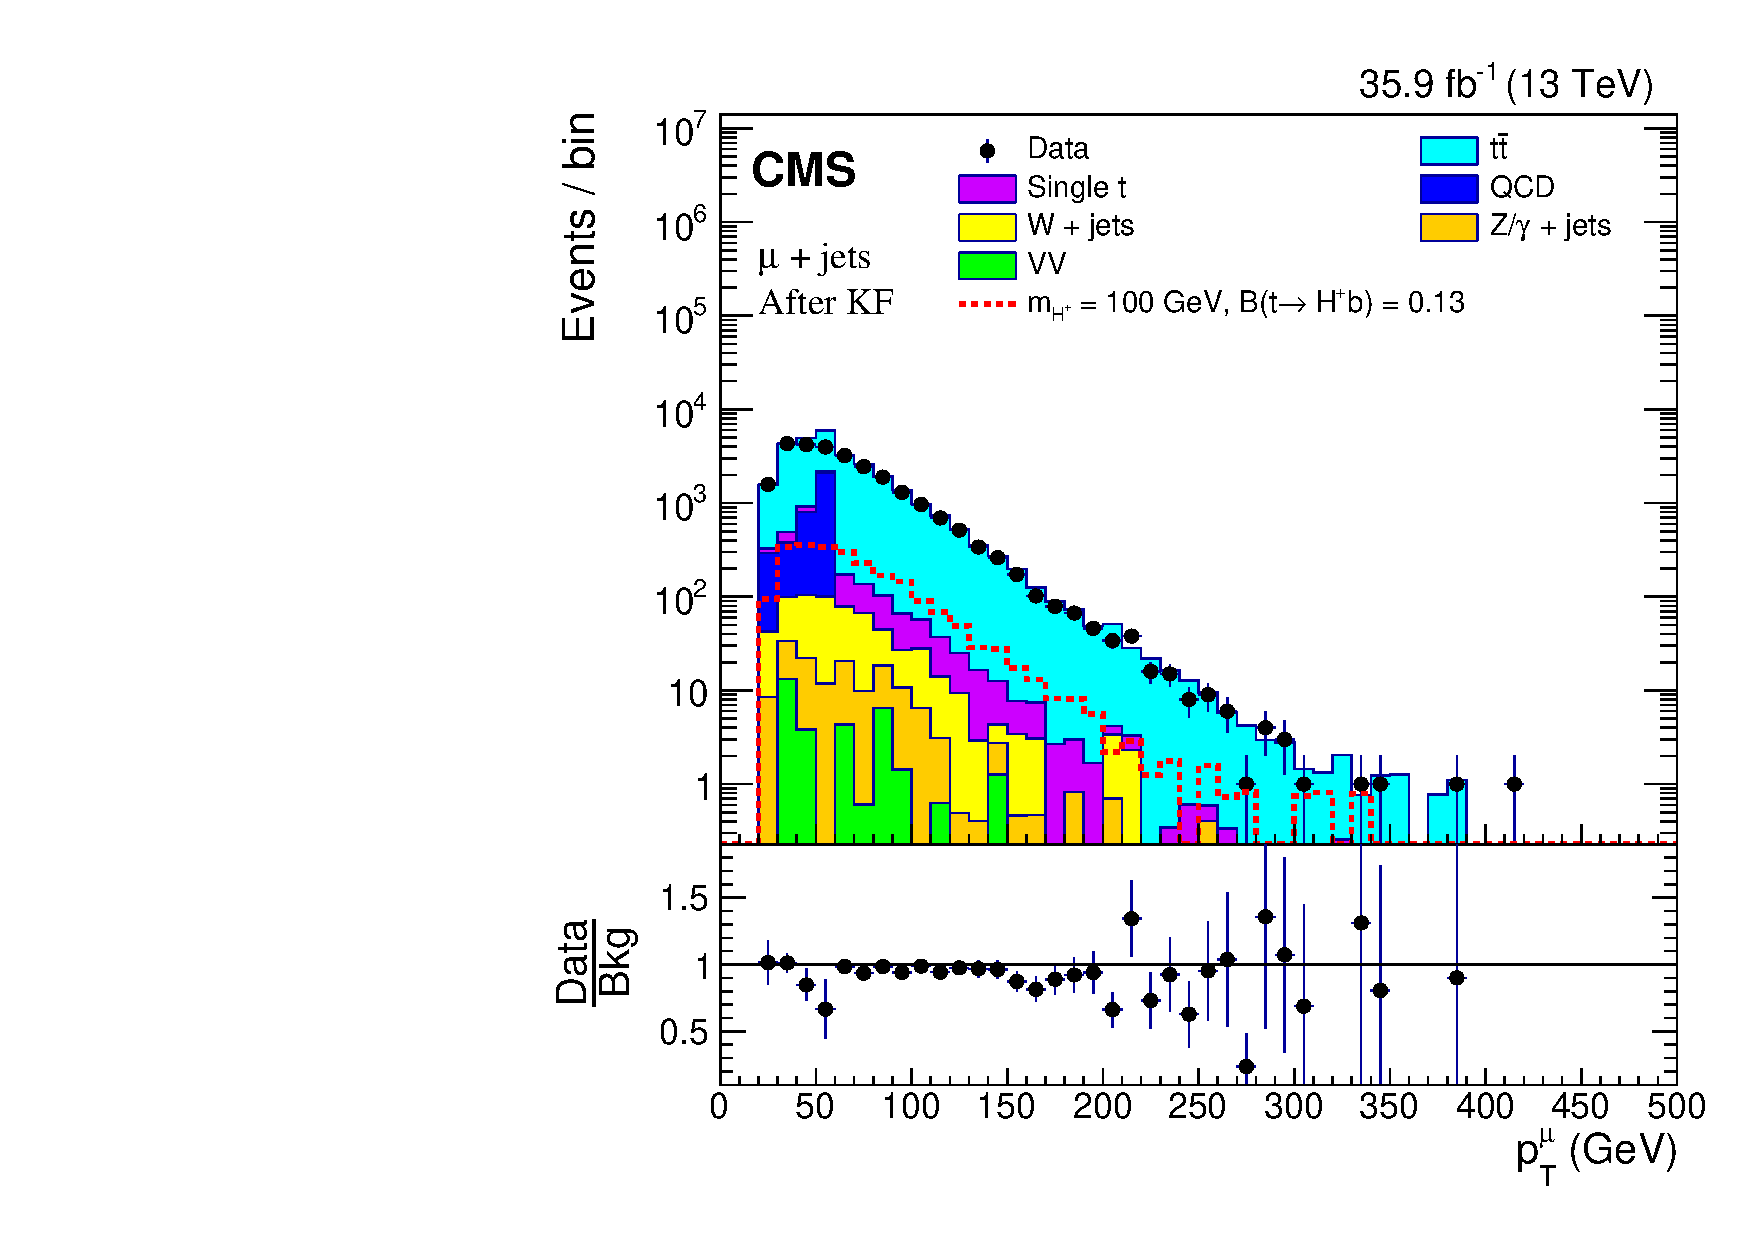
\includegraphics[width=0.45\linewidth]{Image/Muon/LowMET/KinFit/pt_mu_muKinFit.pdf}}
    \subfigure[\pt of electrons]{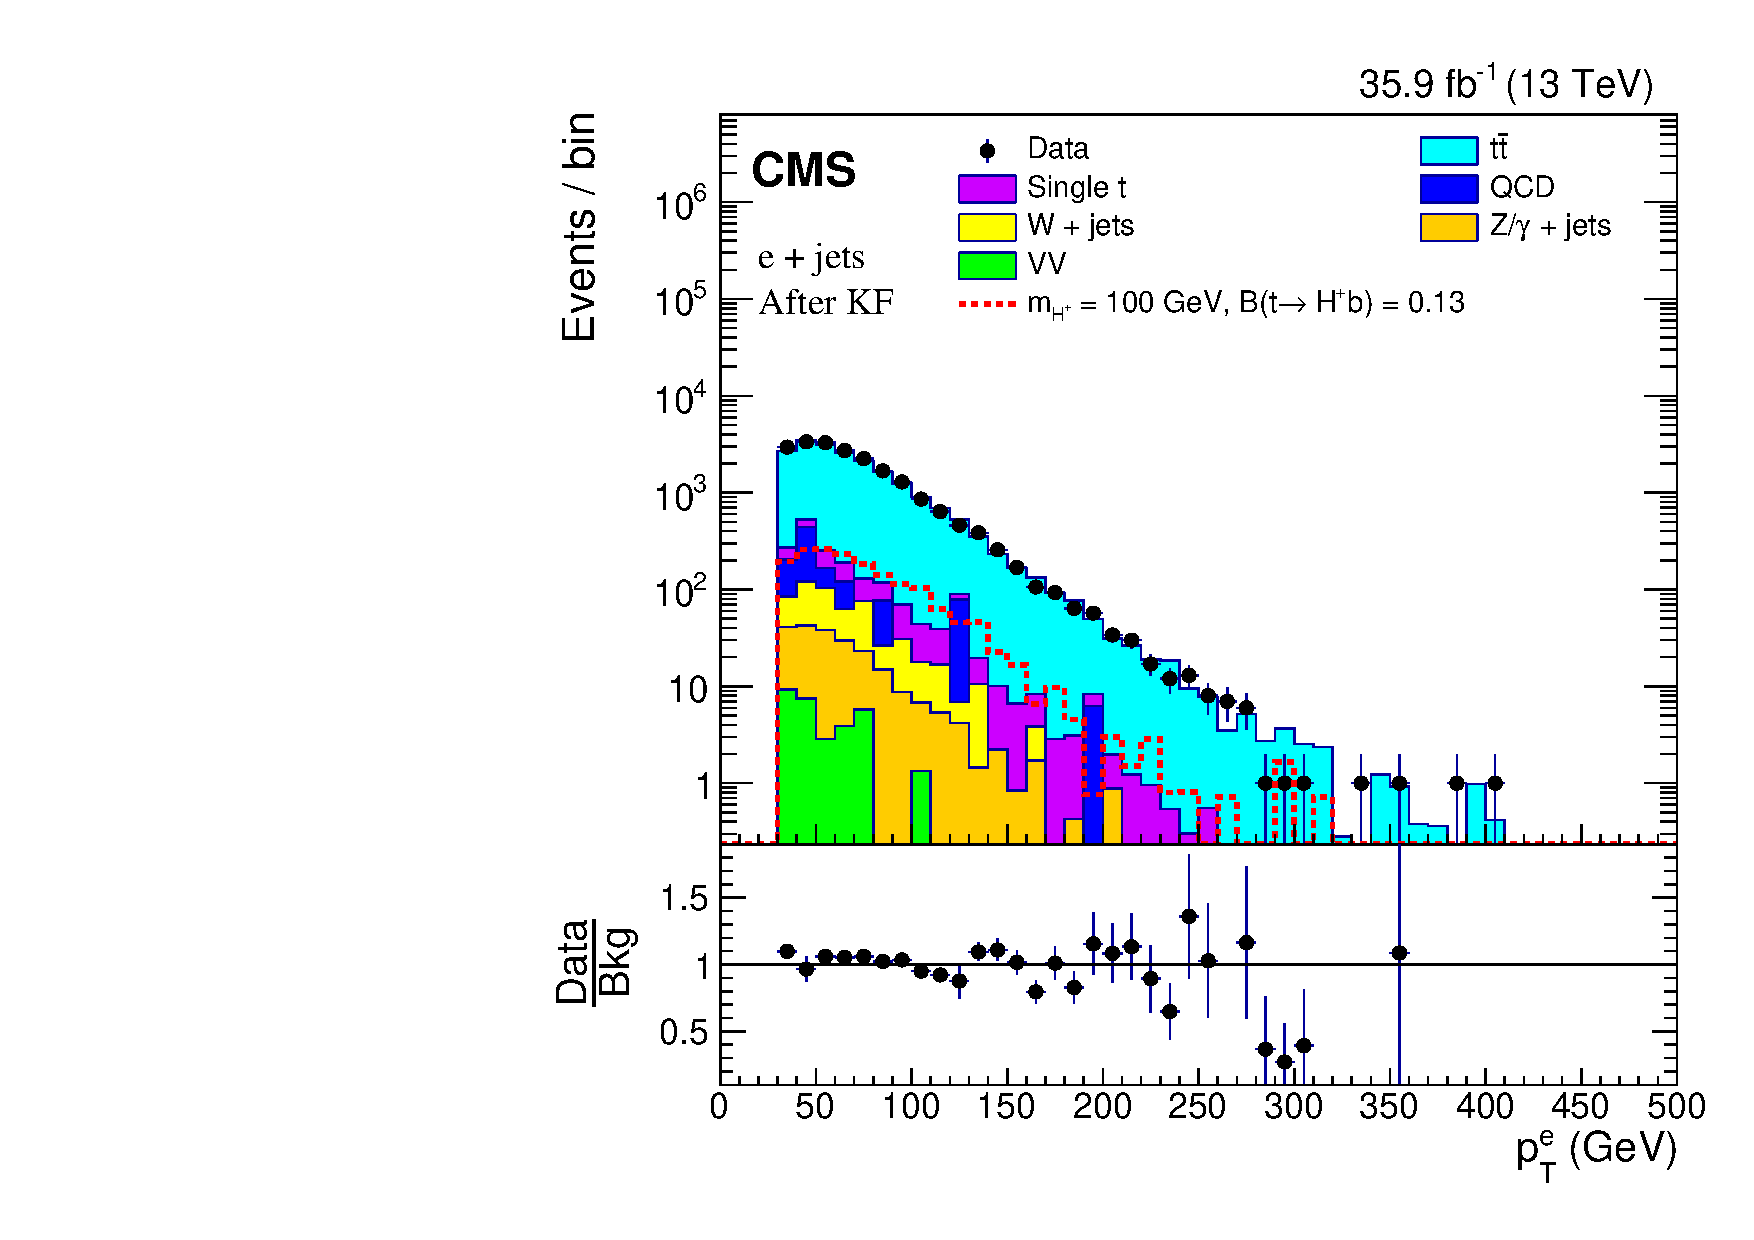
\includegraphics[width=0.45\linewidth]{Image/Electron/LowMET/KinFit/pt_ele_eleKinFit.pdf}}
    \vfil
    \subfigure[$\eta$ of muons]{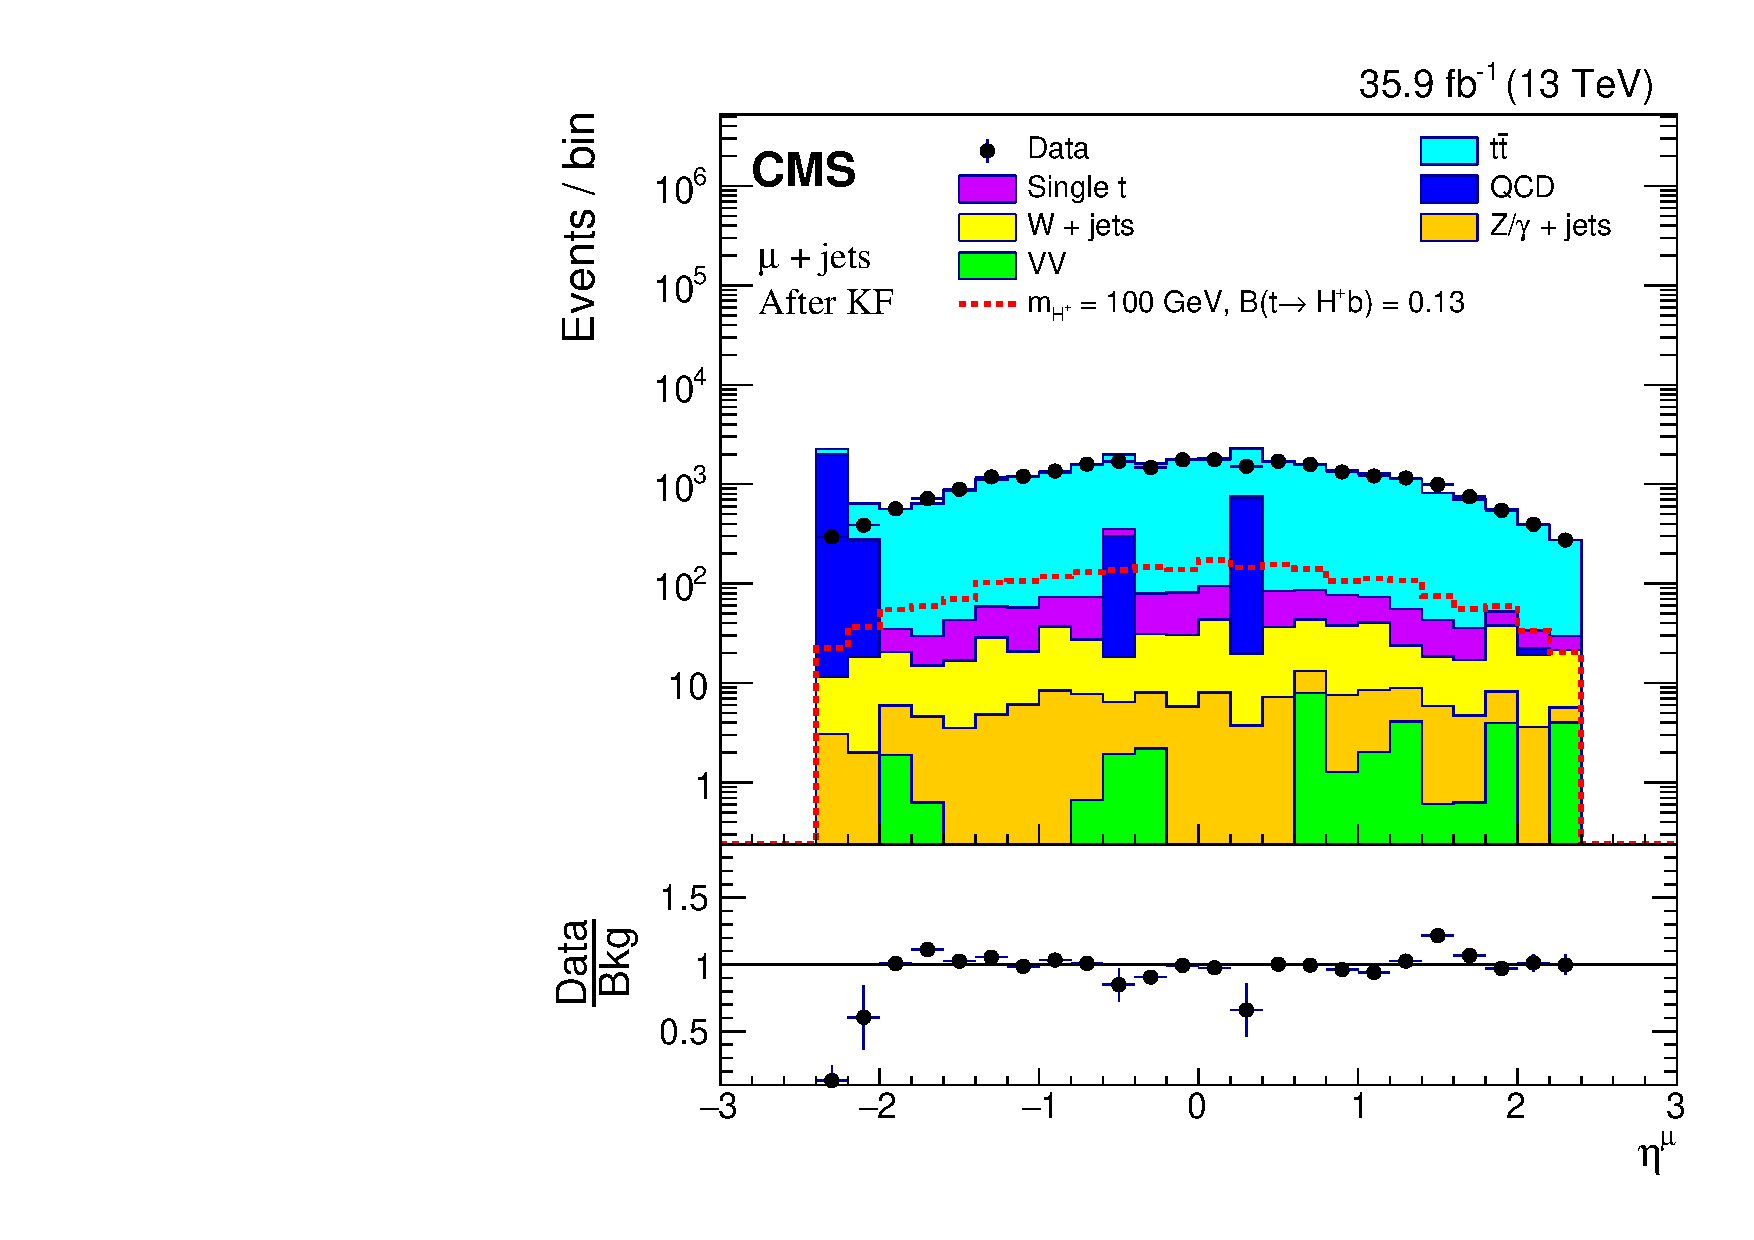
\includegraphics[width=0.45\linewidth]{Image/Muon/LowMET/KinFit/eta_mu_muKinFit.pdf}}
    \subfigure[$\eta$ of electrons]{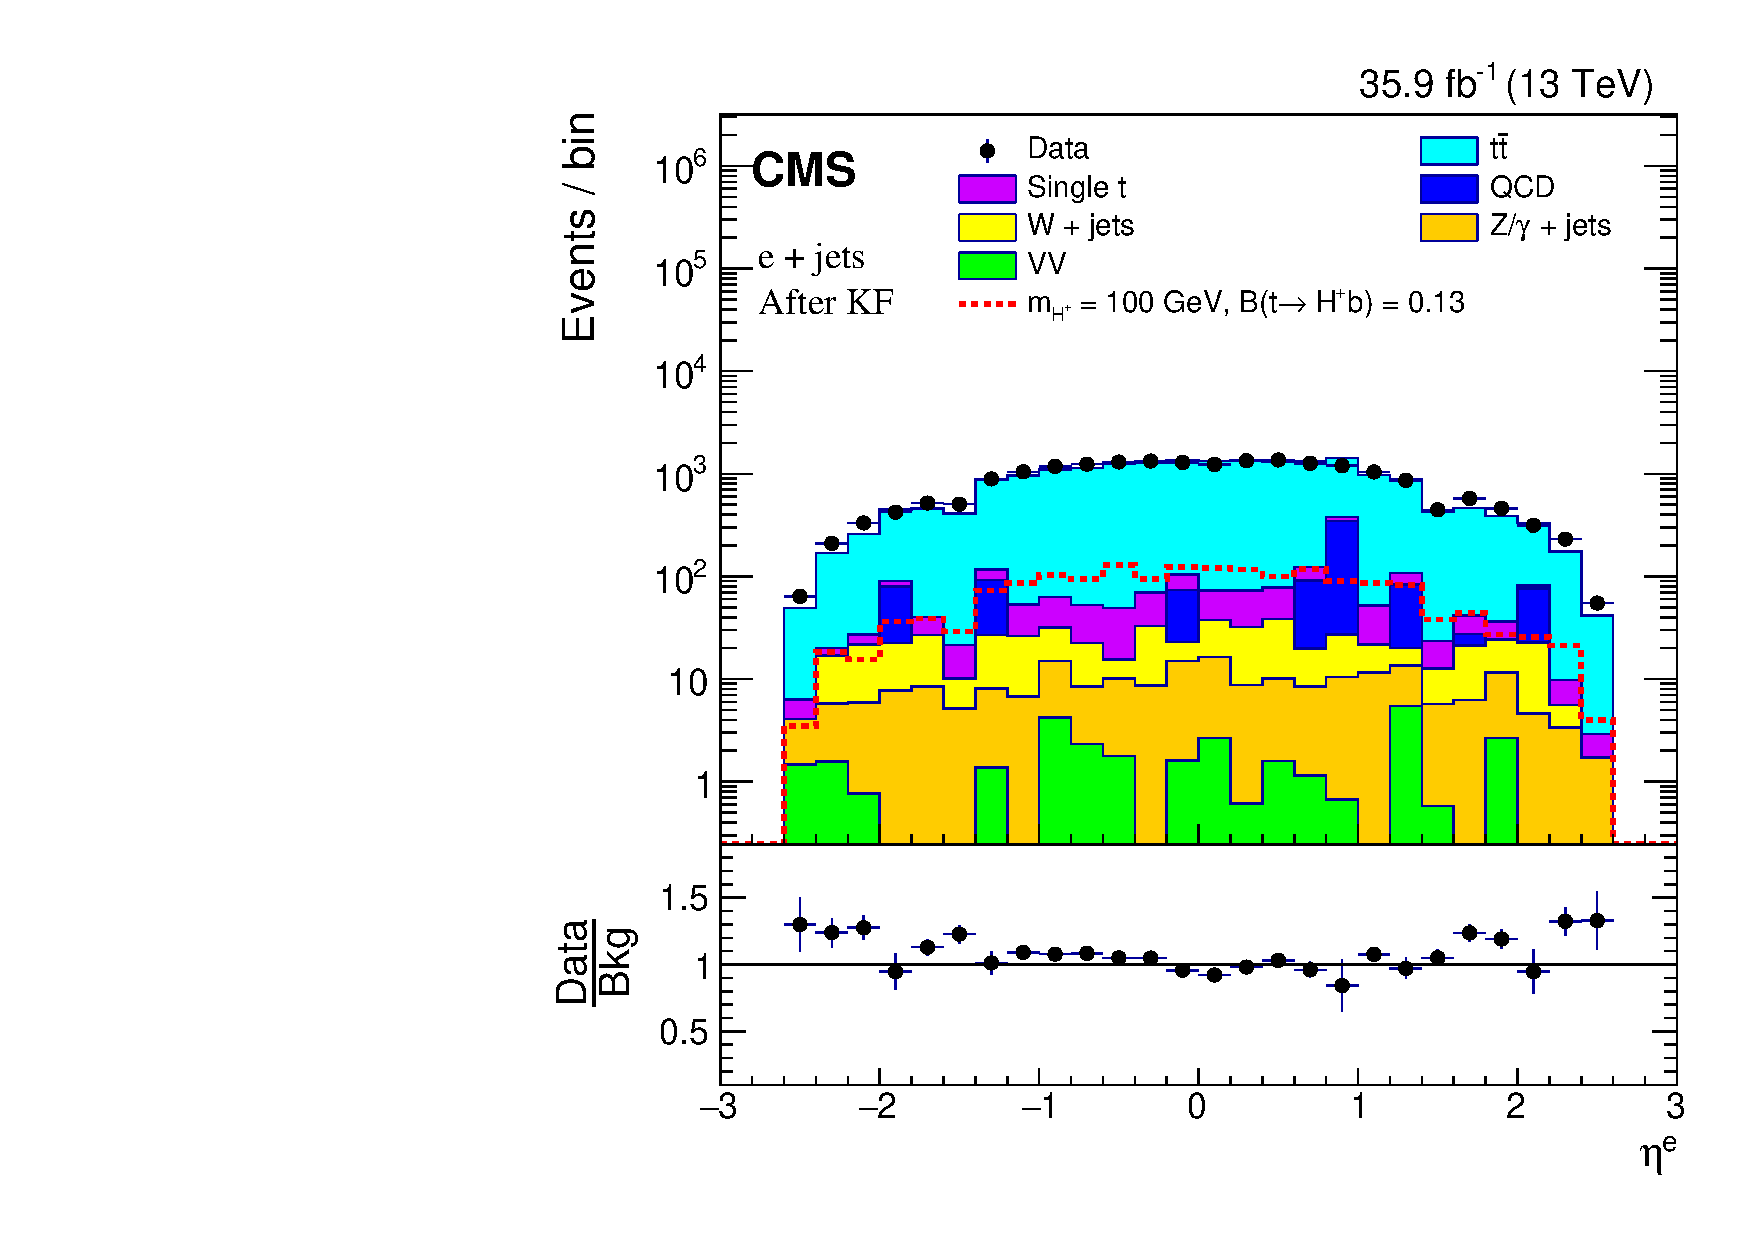
\includegraphics[width=0.45\linewidth]{Image/Electron/LowMET/KinFit/eta_ele_eleKinFit.pdf}}
    \vfil
    \subfigure[\pt of jets]{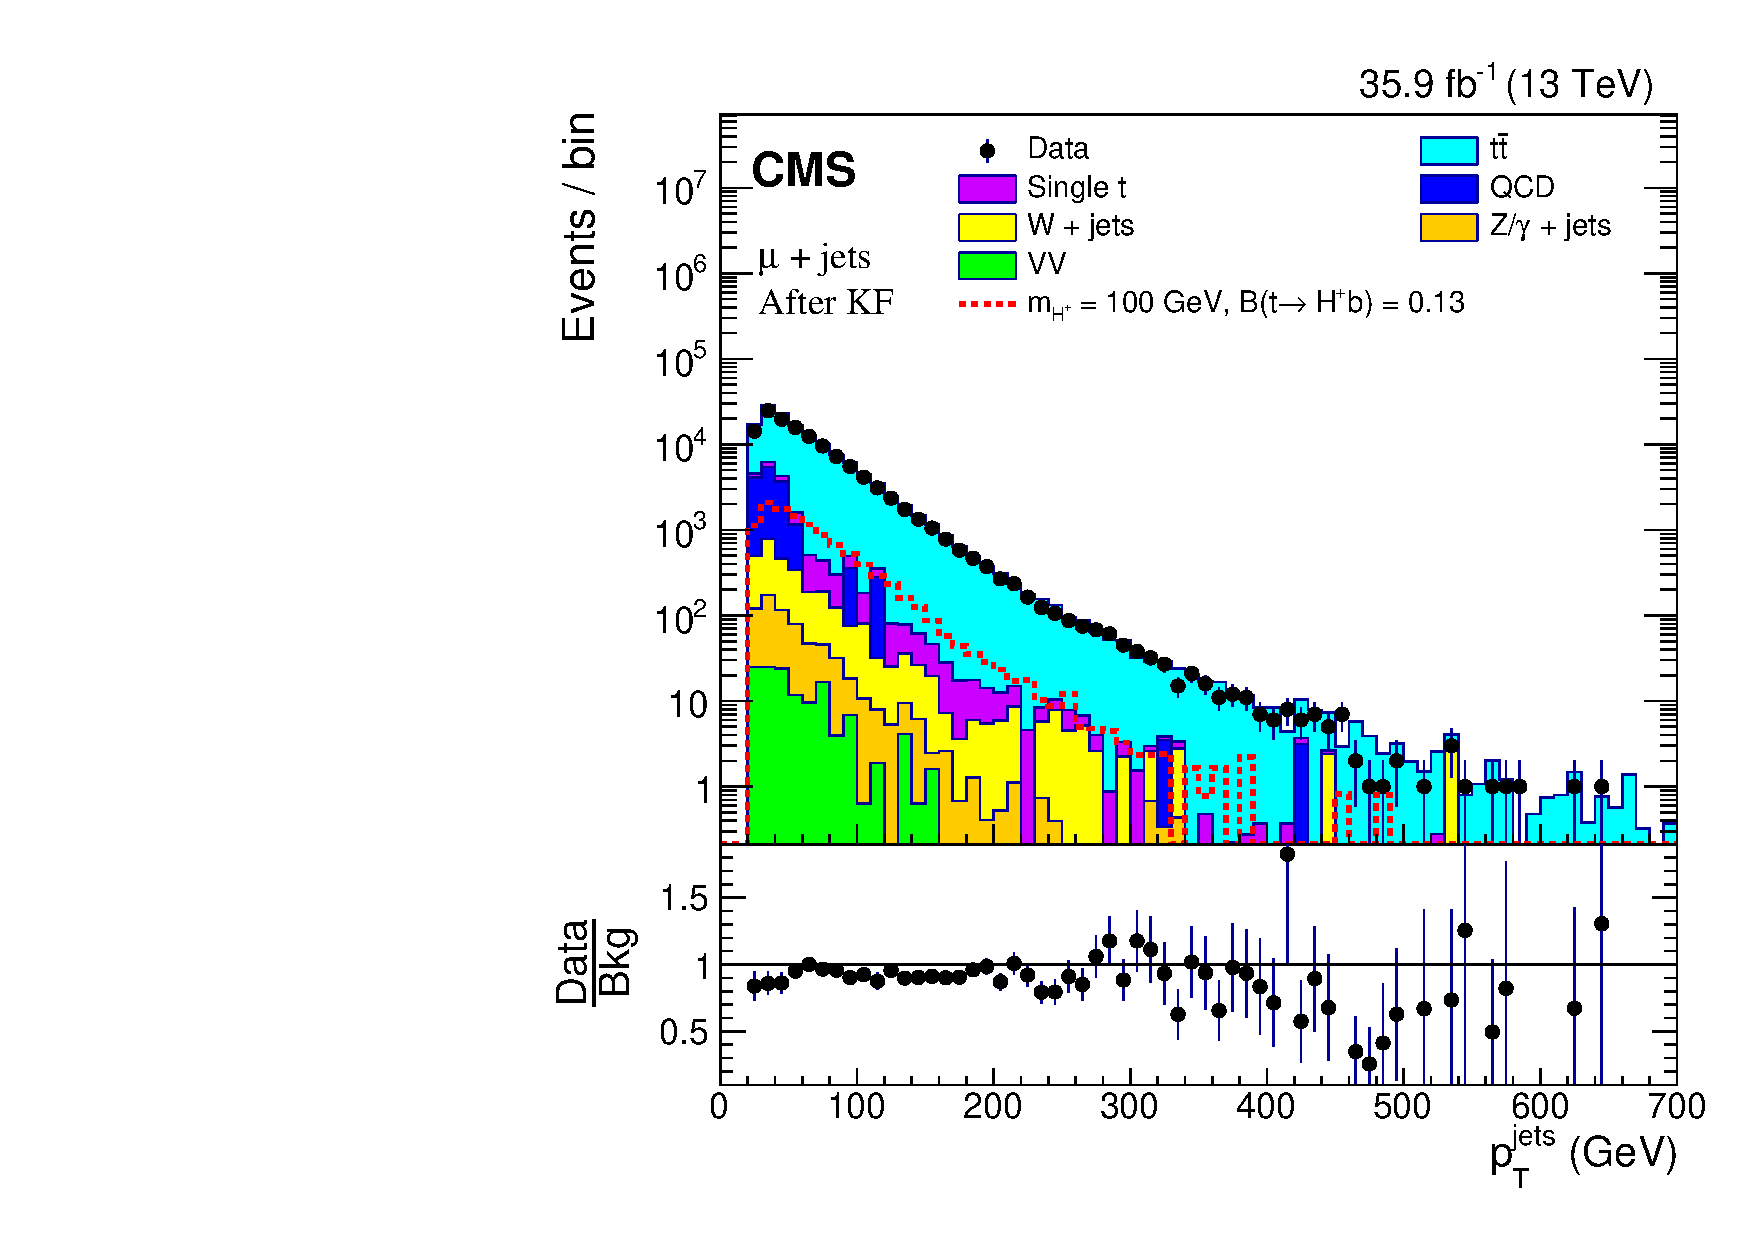
\includegraphics[width=0.45\linewidth]{Image/Muon/LowMET/KinFit/pt_jet_muKinFit.pdf}}
    \subfigure[\pt of jets]{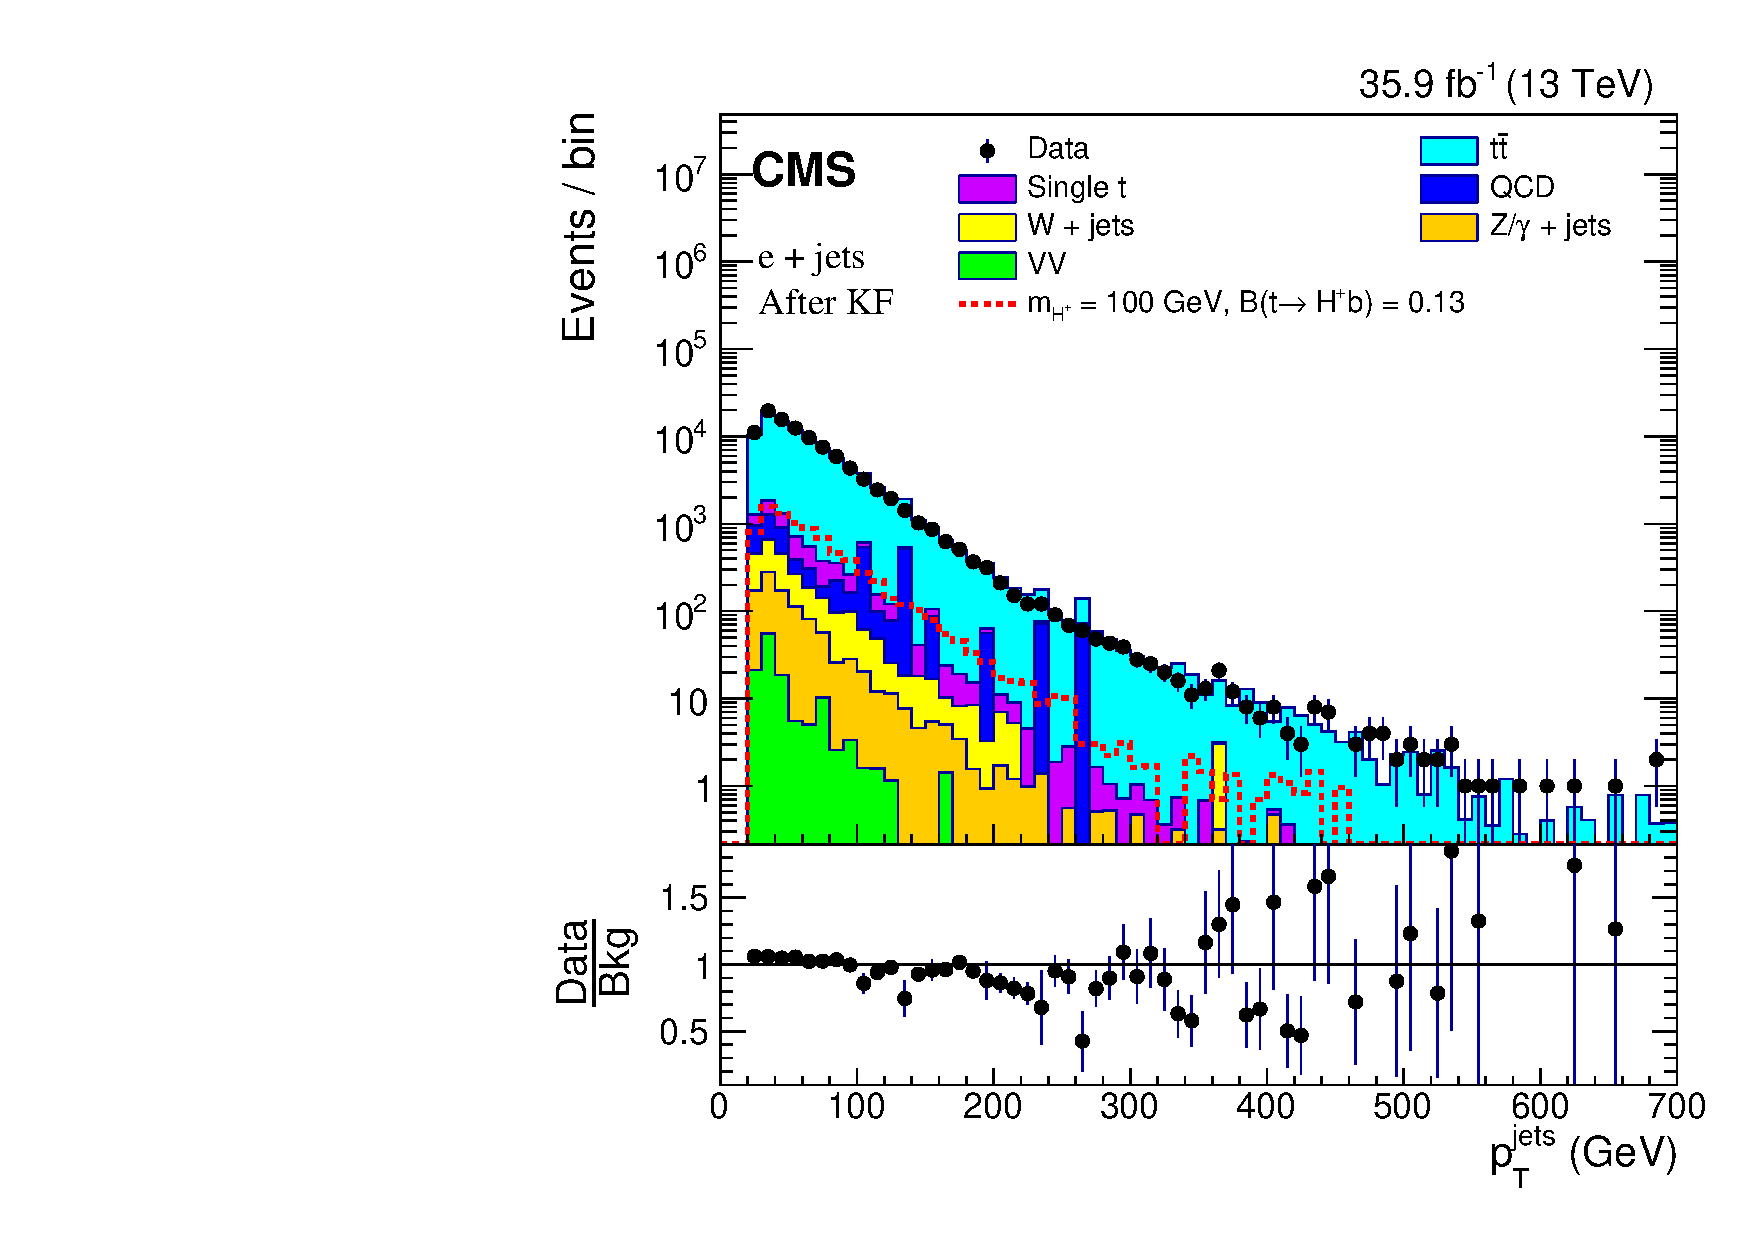
\includegraphics[width=0.45\linewidth]{Image/Electron/LowMET/KinFit/pt_jet_eleKinFit.pdf}}
    \caption{Control plots in $\MET <$ 20 GeV region, after kinematic fit selection as described in Sec.~\ref{s:secEvtSel}, 
for muons + jets and \ejets channel.}
    \label{fig:LowMET_kfitPlot1}
\end{figure}

%After KinFit: \MET, MT, N_jets, N_bjets
\begin{figure}
    \centering  
    \subfigure[$\eta$ of jets]{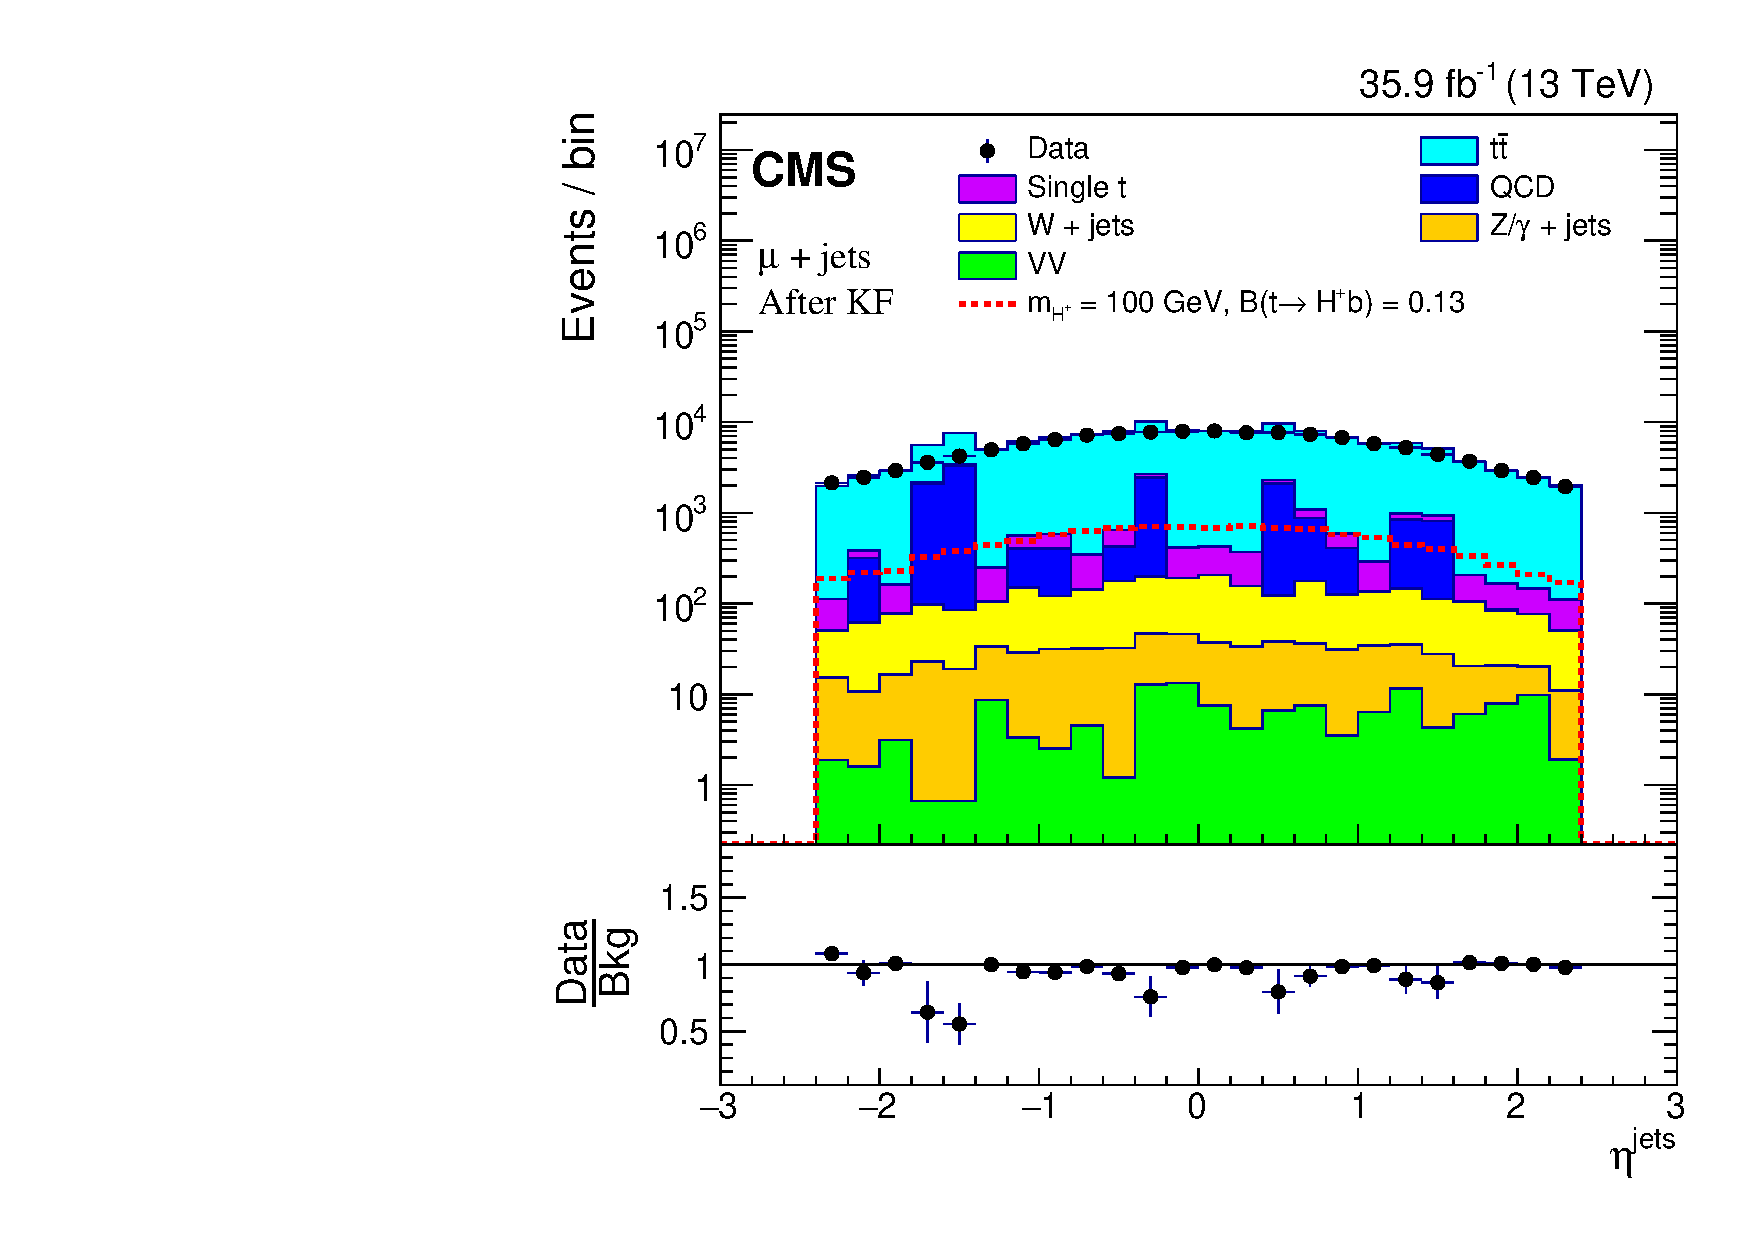
\includegraphics[width=0.45\linewidth]{Image/Muon/LowMET/KinFit/eta_jet_muKinFit.pdf}}
    \subfigure[$\eta$ of jets]{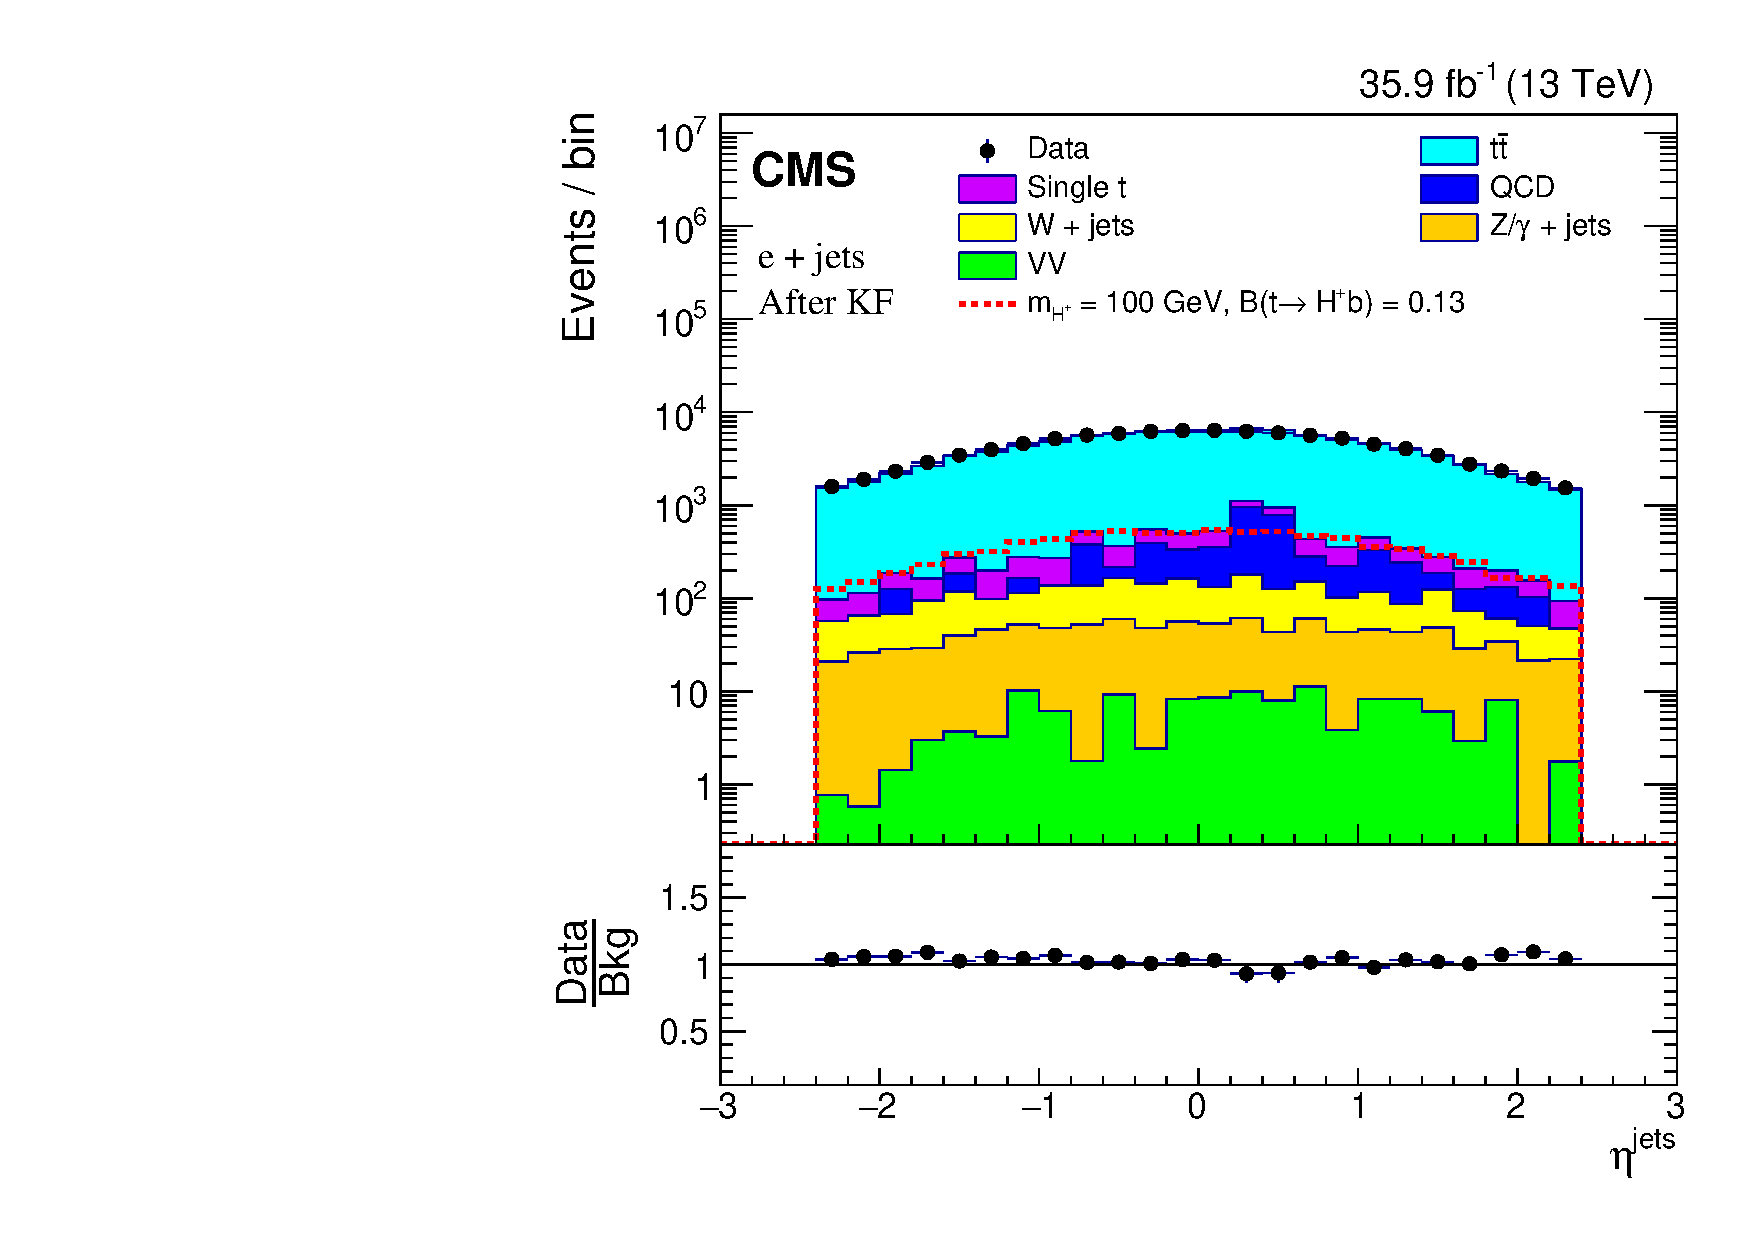
\includegraphics[width=0.45\linewidth]{Image/Electron/LowMET/KinFit/eta_jet_eleKinFit.pdf}}
    \vfil
    \subfigure[jet multiplicity]{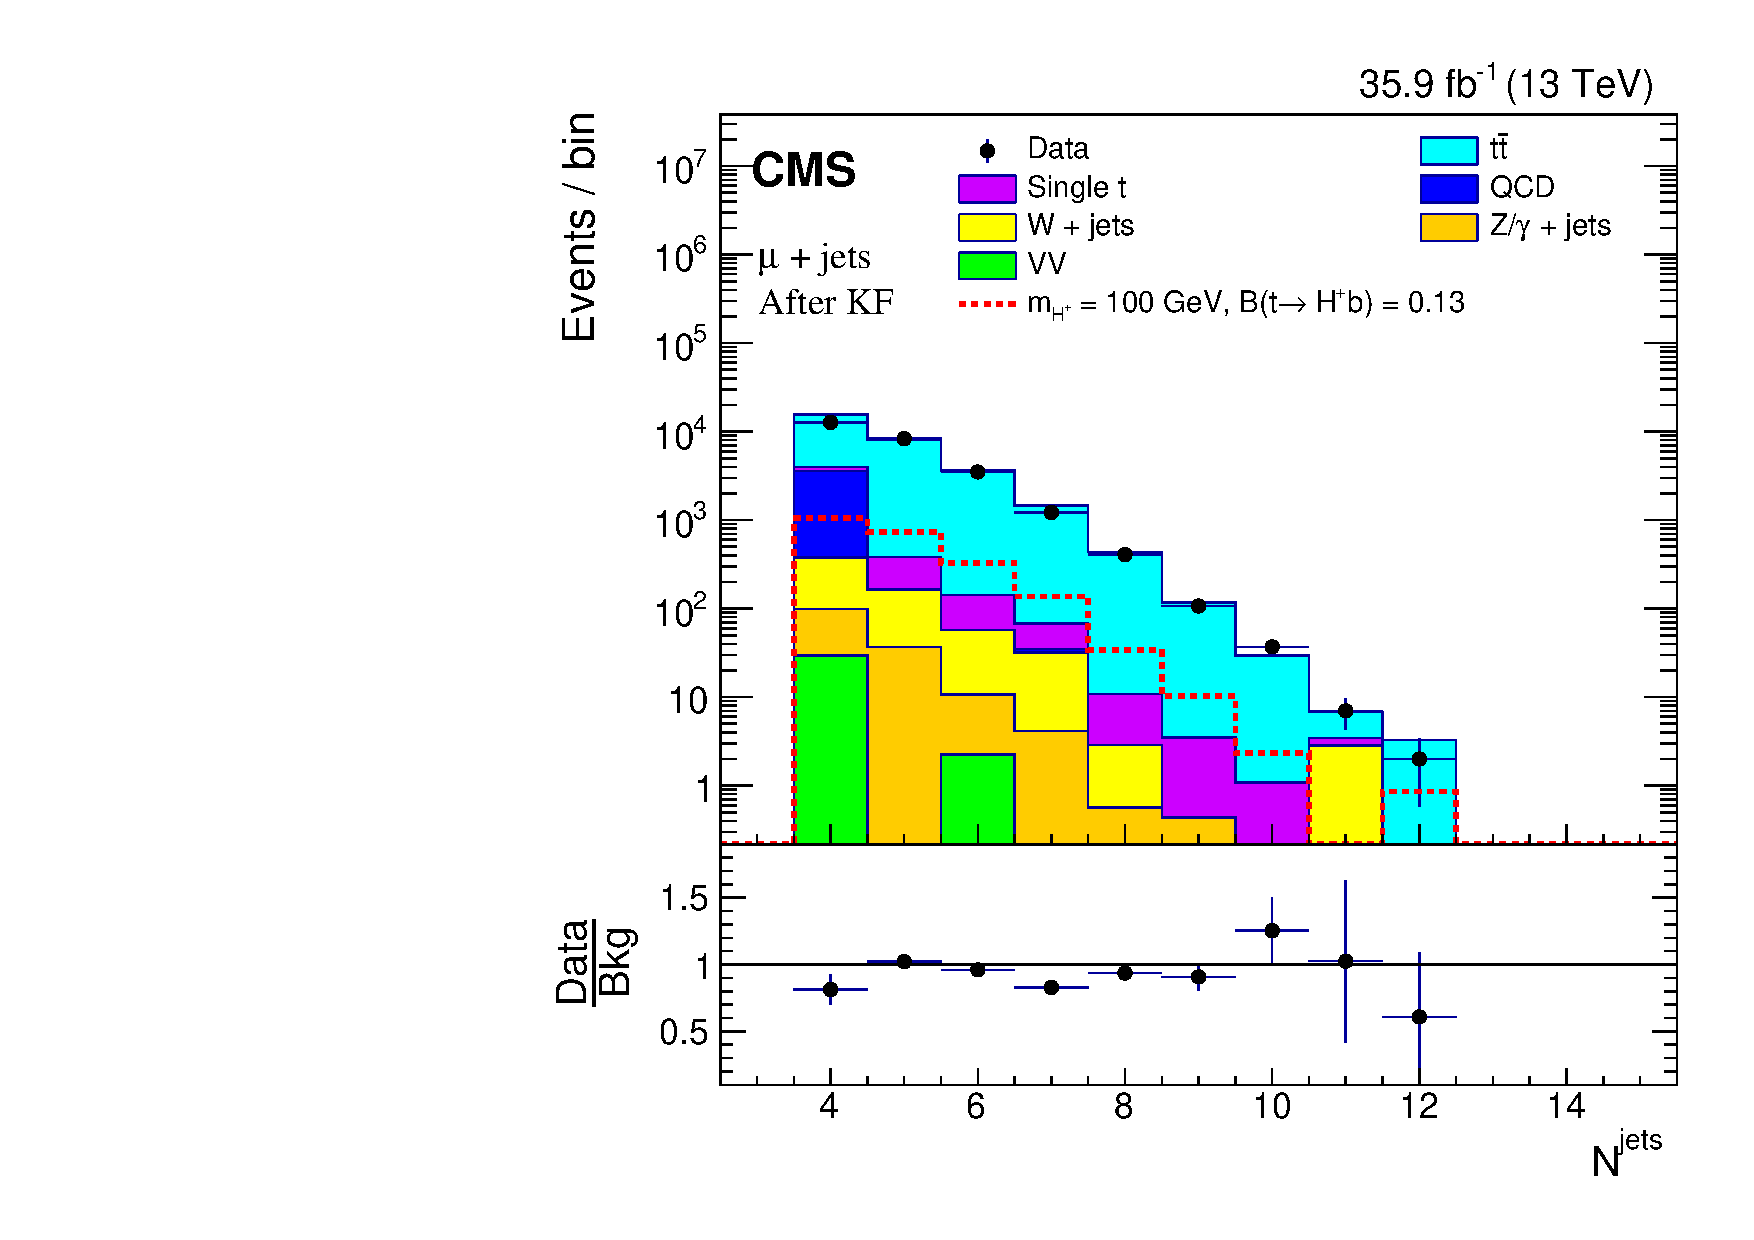
\includegraphics[width=0.45\linewidth]{Image/Muon/LowMET/KinFit/final_multi_jet_muKinFit.pdf}}
    \subfigure[jet multiplicity]{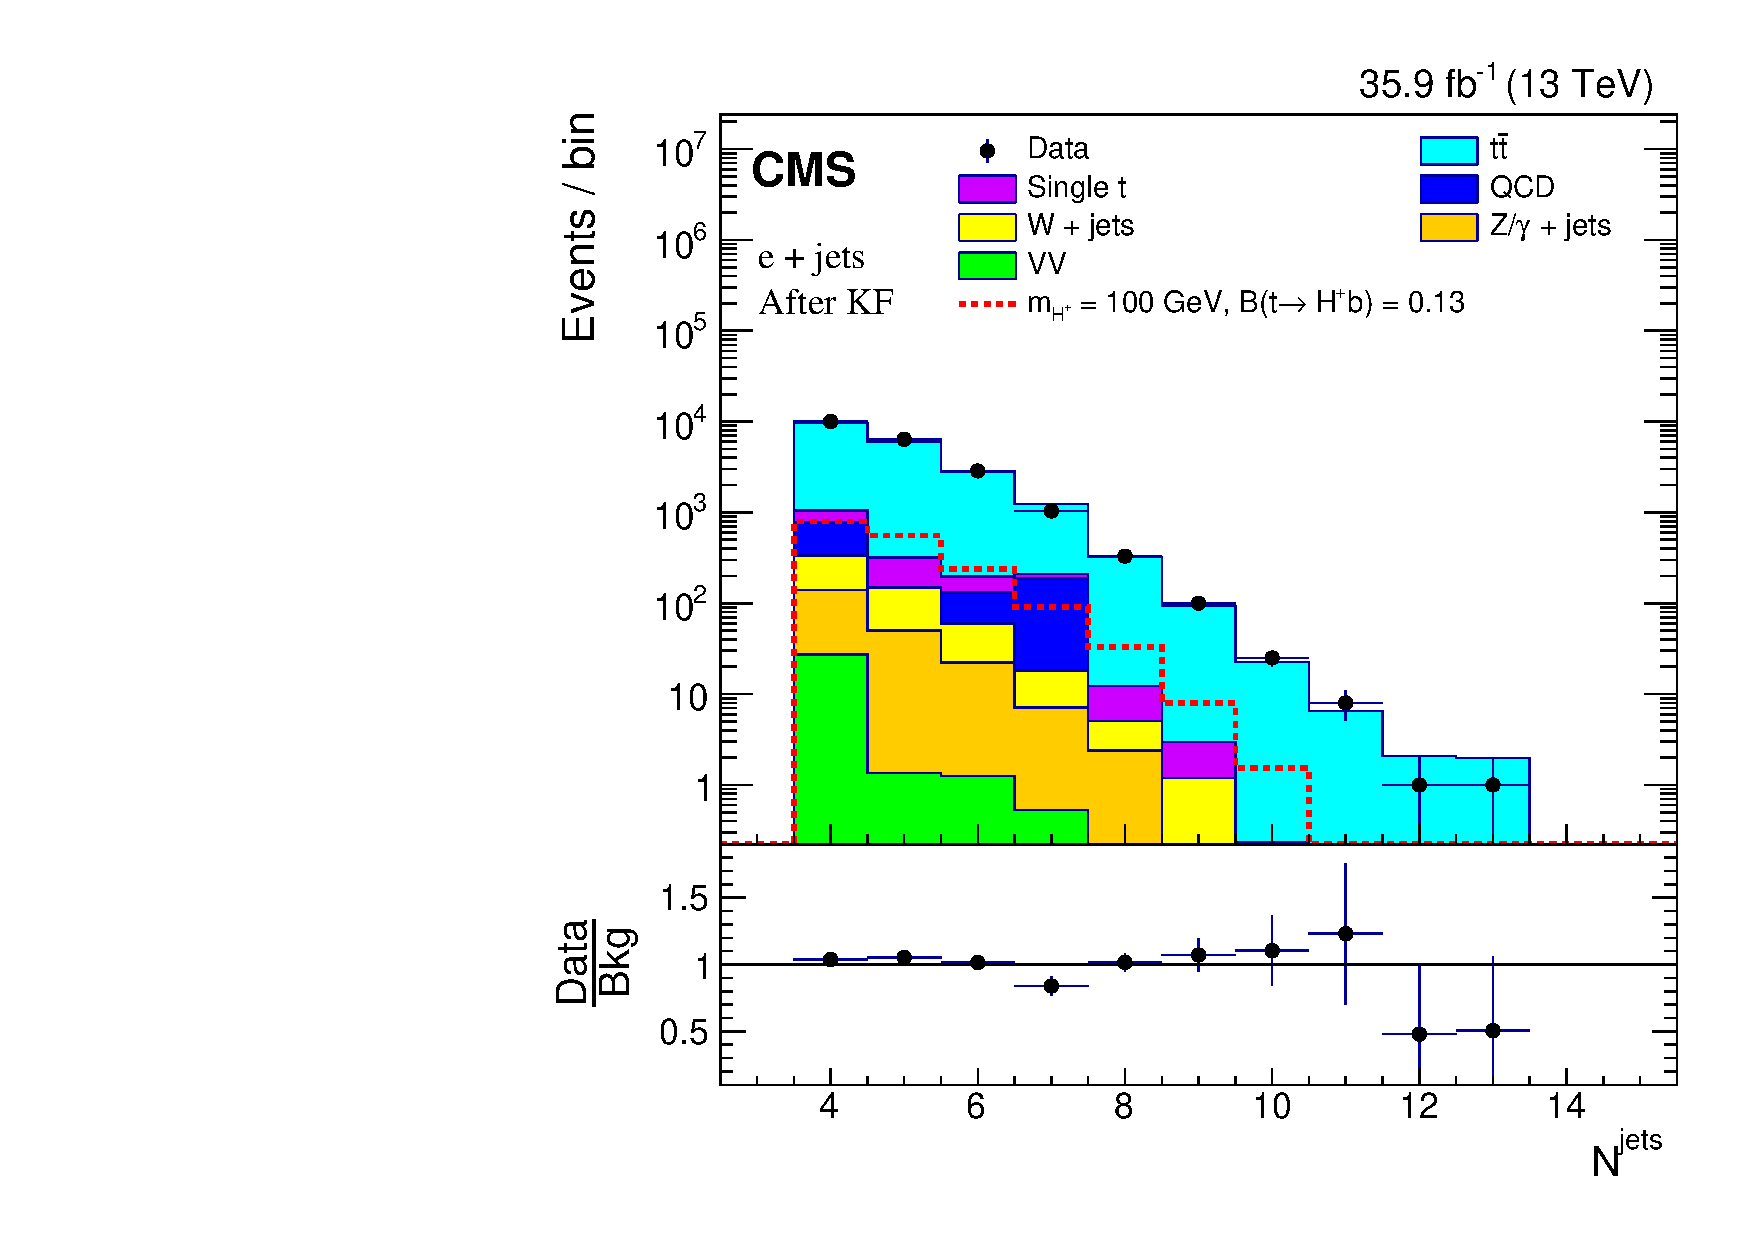
\includegraphics[width=0.45\linewidth]{Image/Electron/LowMET/KinFit/final_multi_jet_eleKinFit.pdf}}
    \vfil
    \subfigure[b-jet multiplicity]{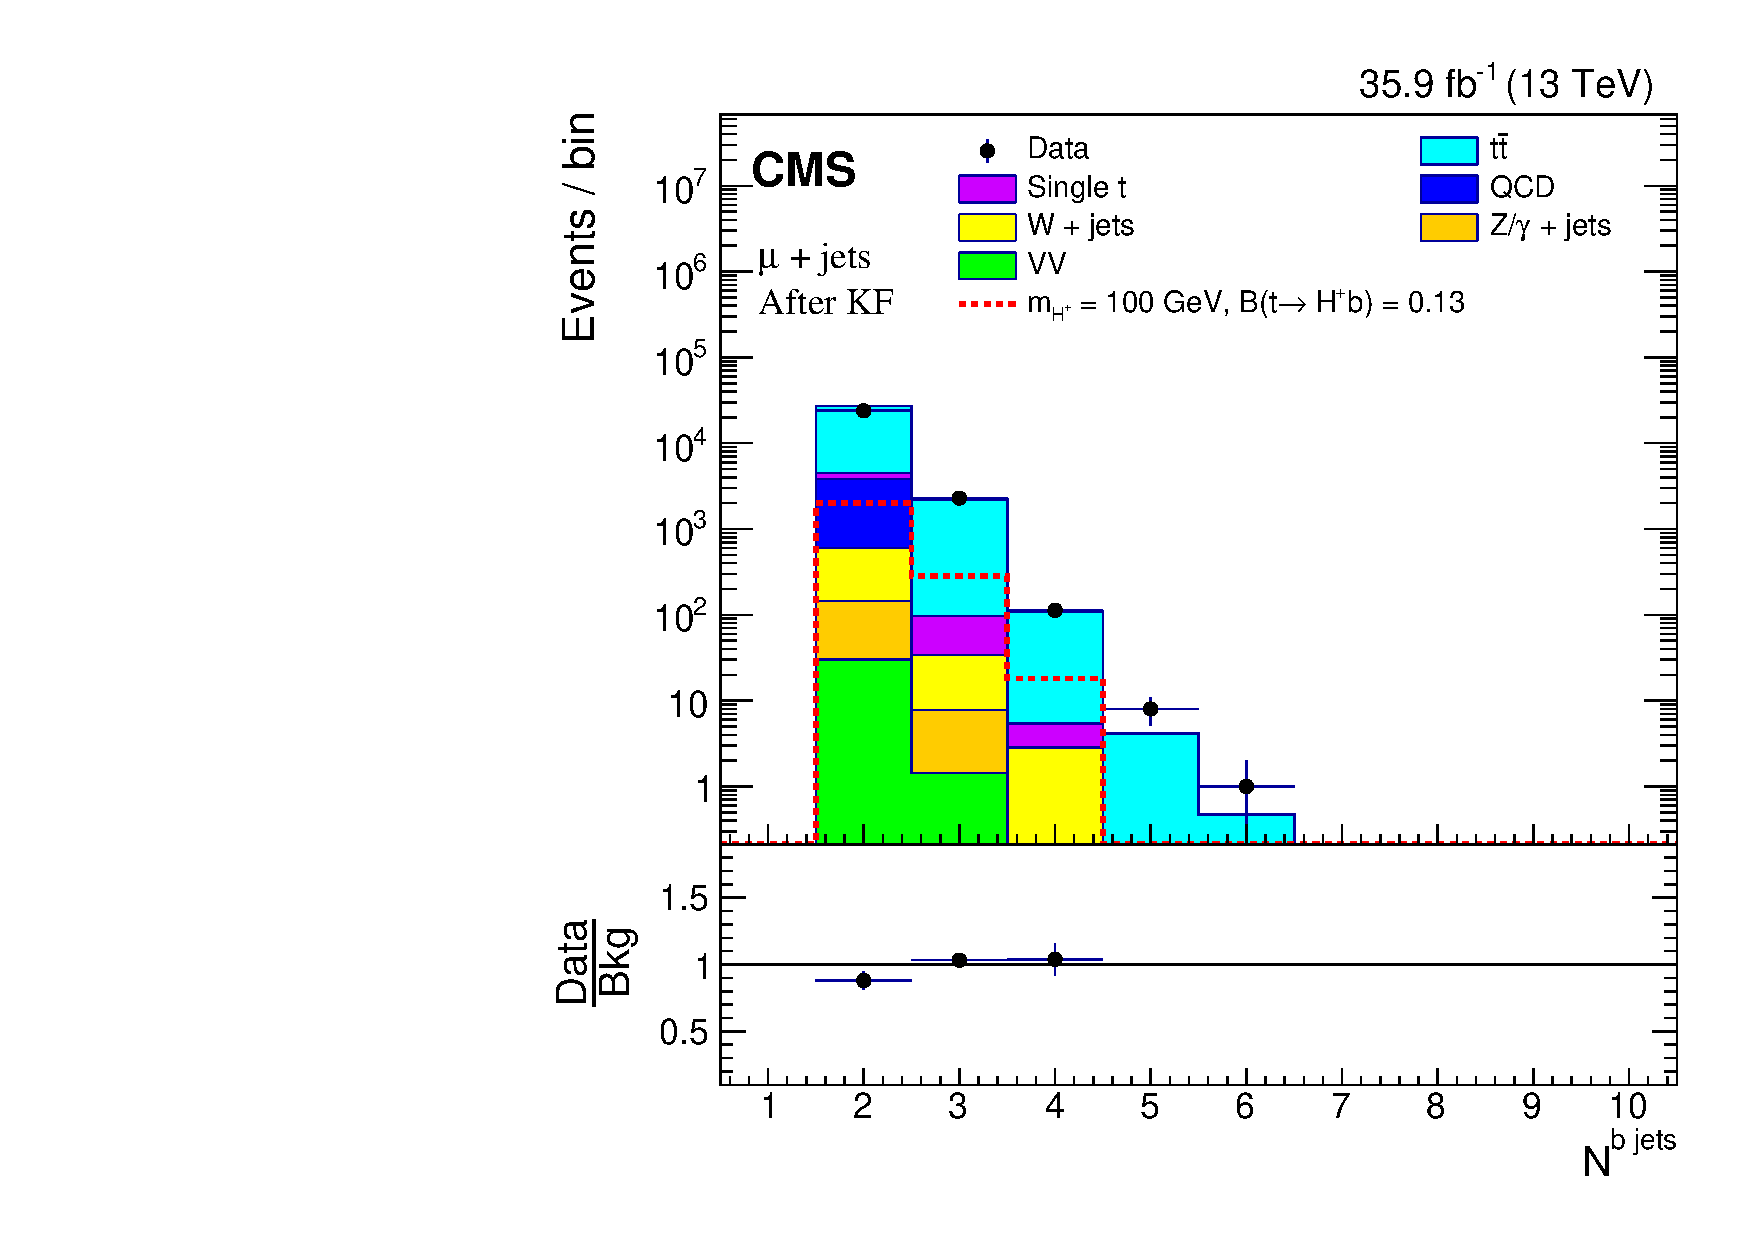
\includegraphics[width=0.45\linewidth]{Image/Muon/LowMET/KinFit/CSVL_count_muKinFit.pdf}}
    \subfigure[b-jet multiplicity]{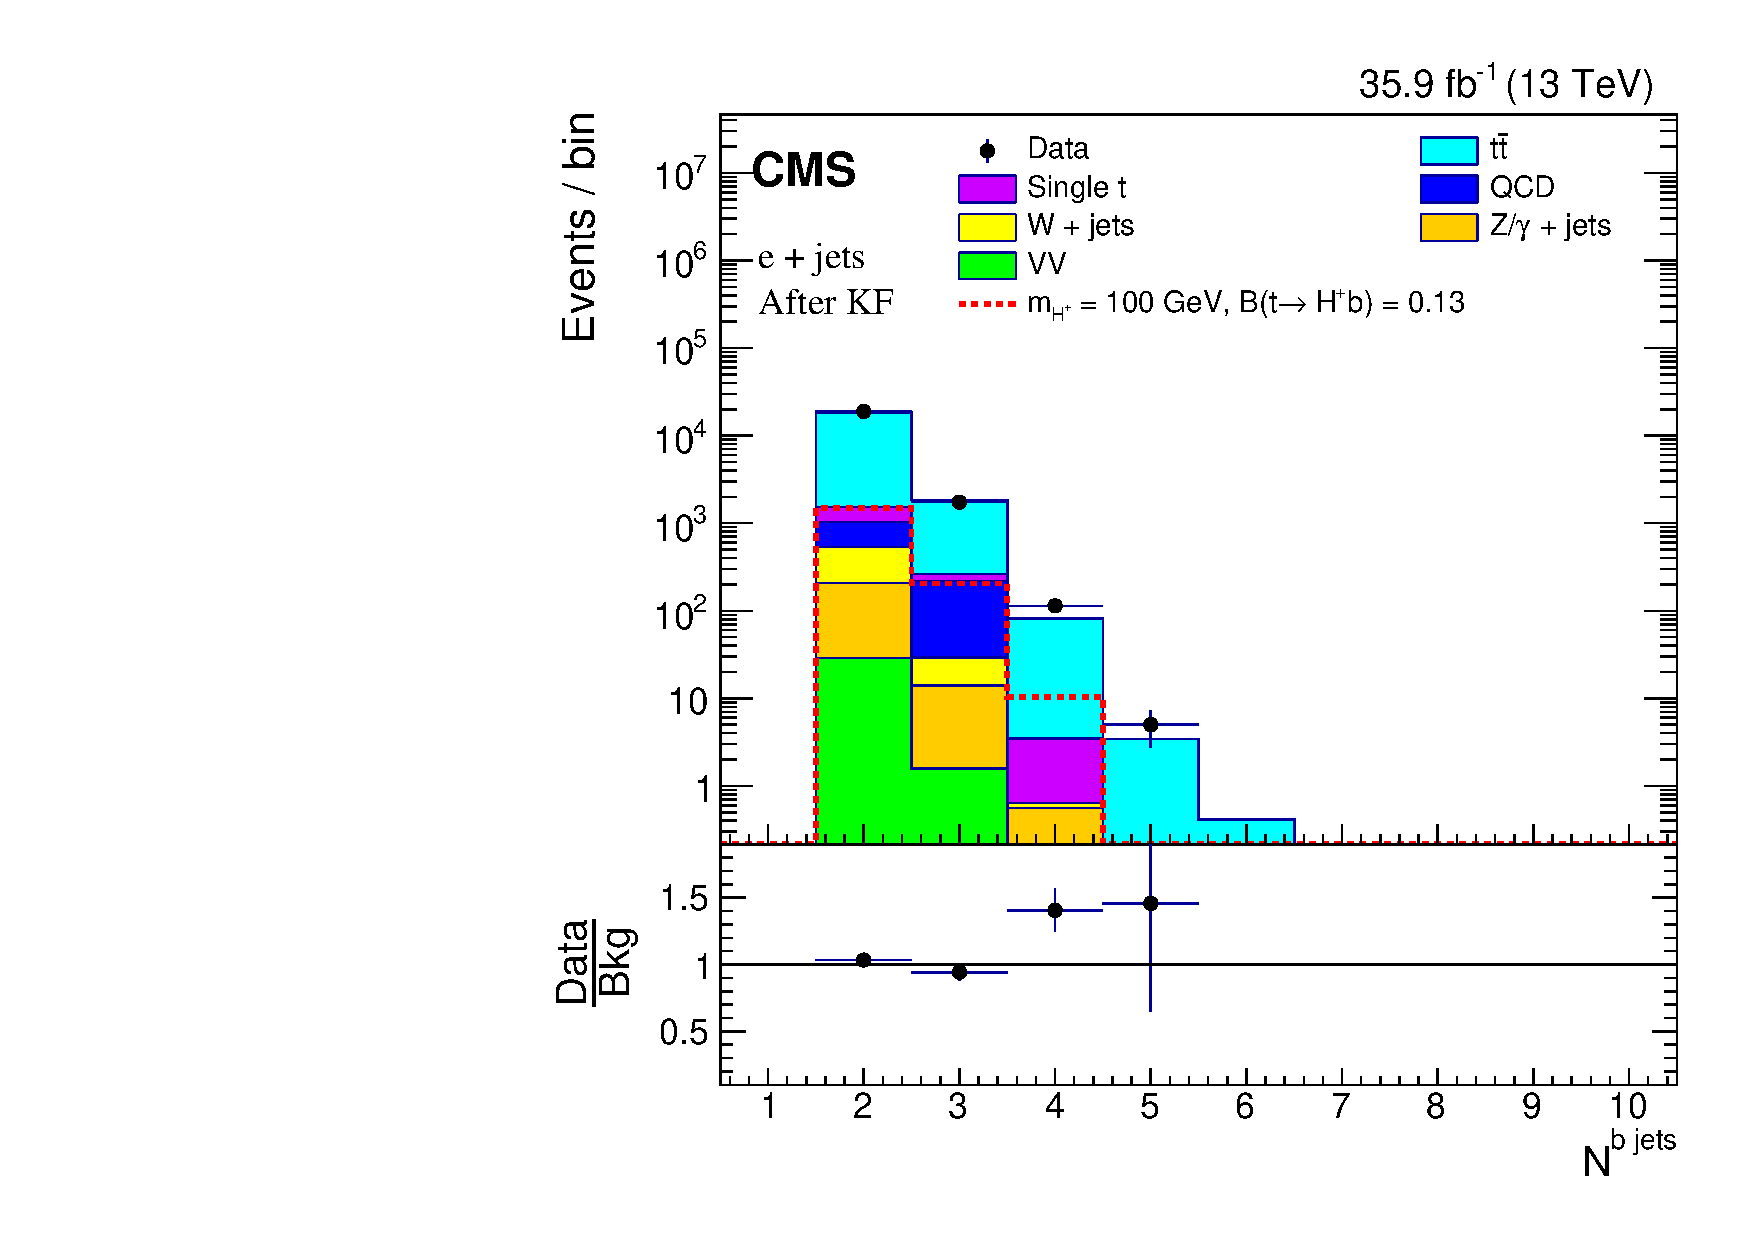
\includegraphics[width=0.45\linewidth]{Image/Electron/LowMET/KinFit/CSVL_count_eleKinFit.pdf}}
    \caption{Control plots in $\MET <$ 20 GeV region, after kinematic fit selection as described
        in Sec.~\ref{s:secEvtSel}, for muons + jets and \ejets
    channel.}
    \label{fig:LowMET_kfitPlot2}
\end{figure}

\begin{figure}
    \centering  
    \subfigure[\MET]{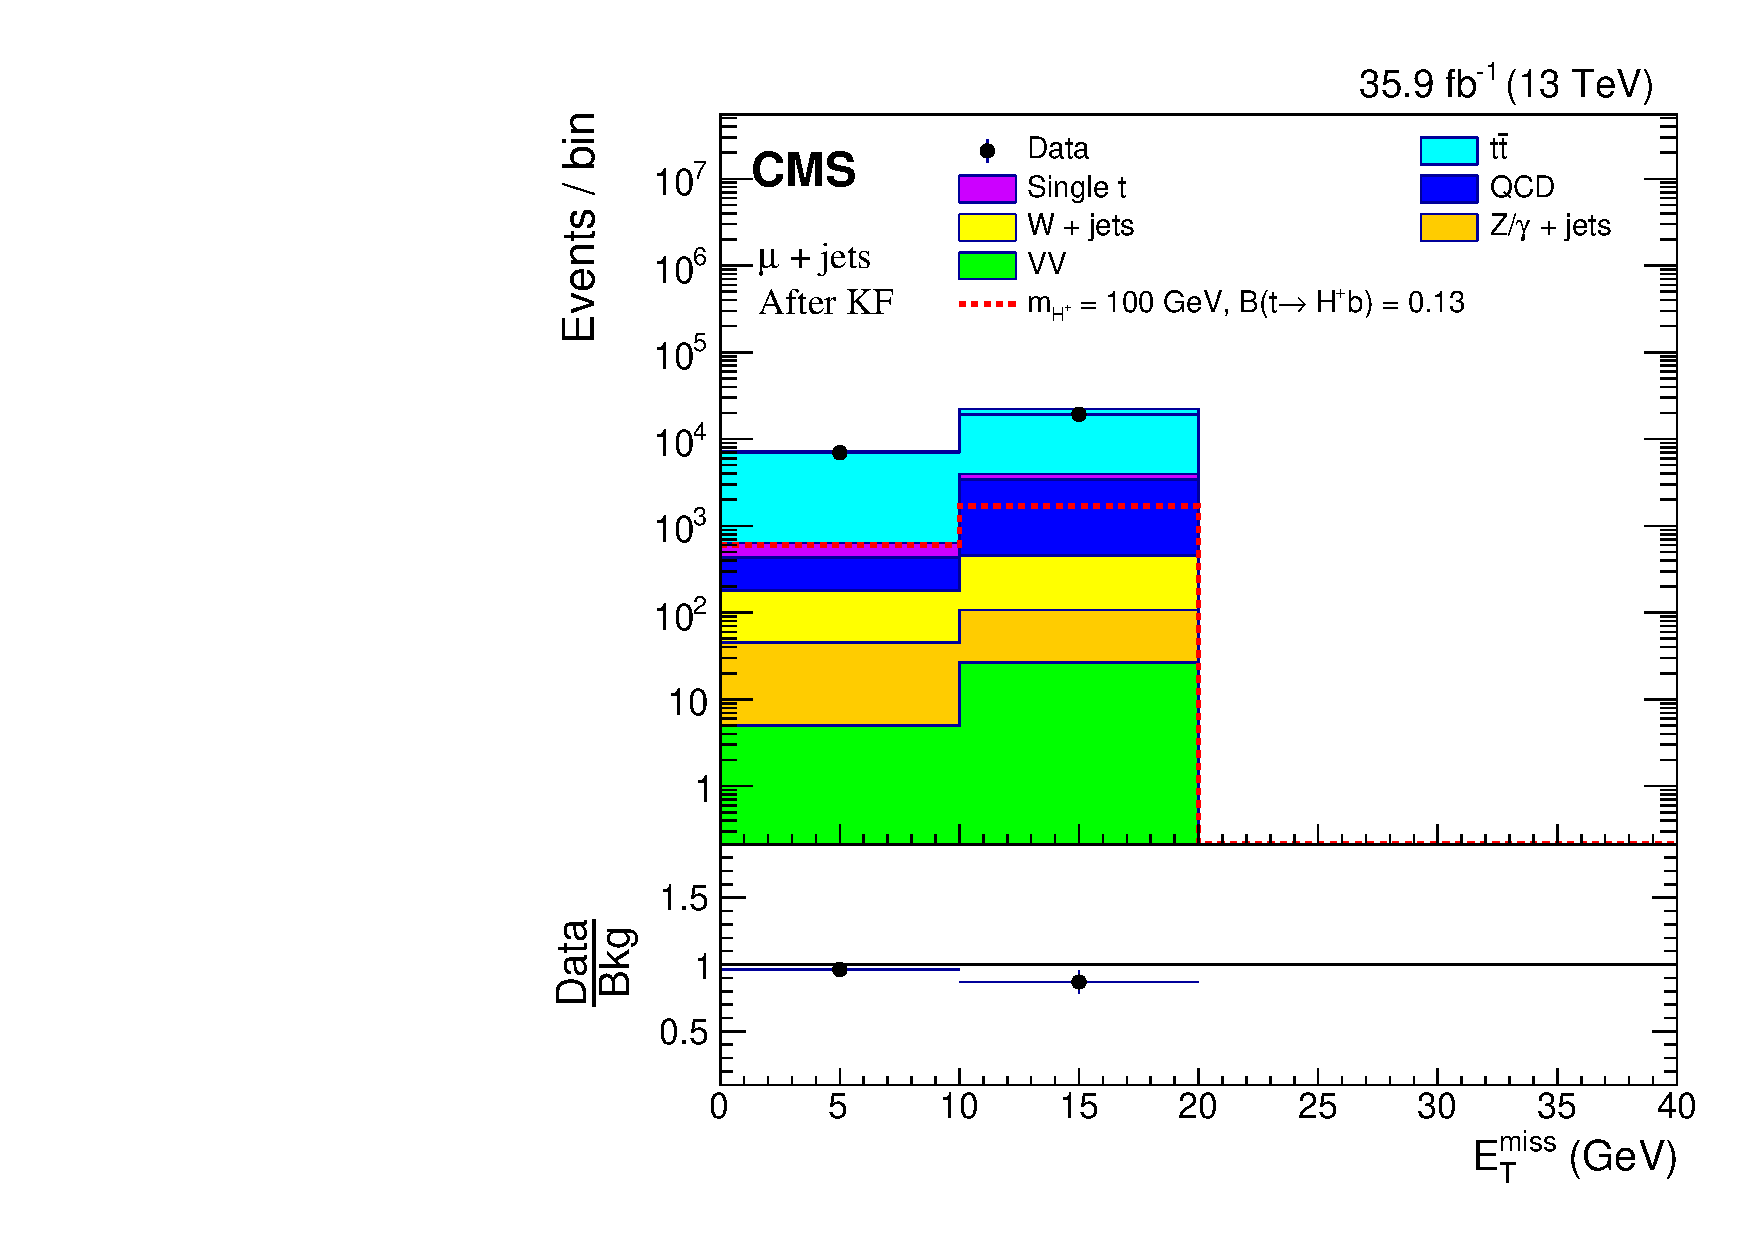
\includegraphics[width=0.45\linewidth]{Image/Muon/LowMET/KinFit/final_pt_met_muKinFit.pdf}}
    \subfigure[\MET]{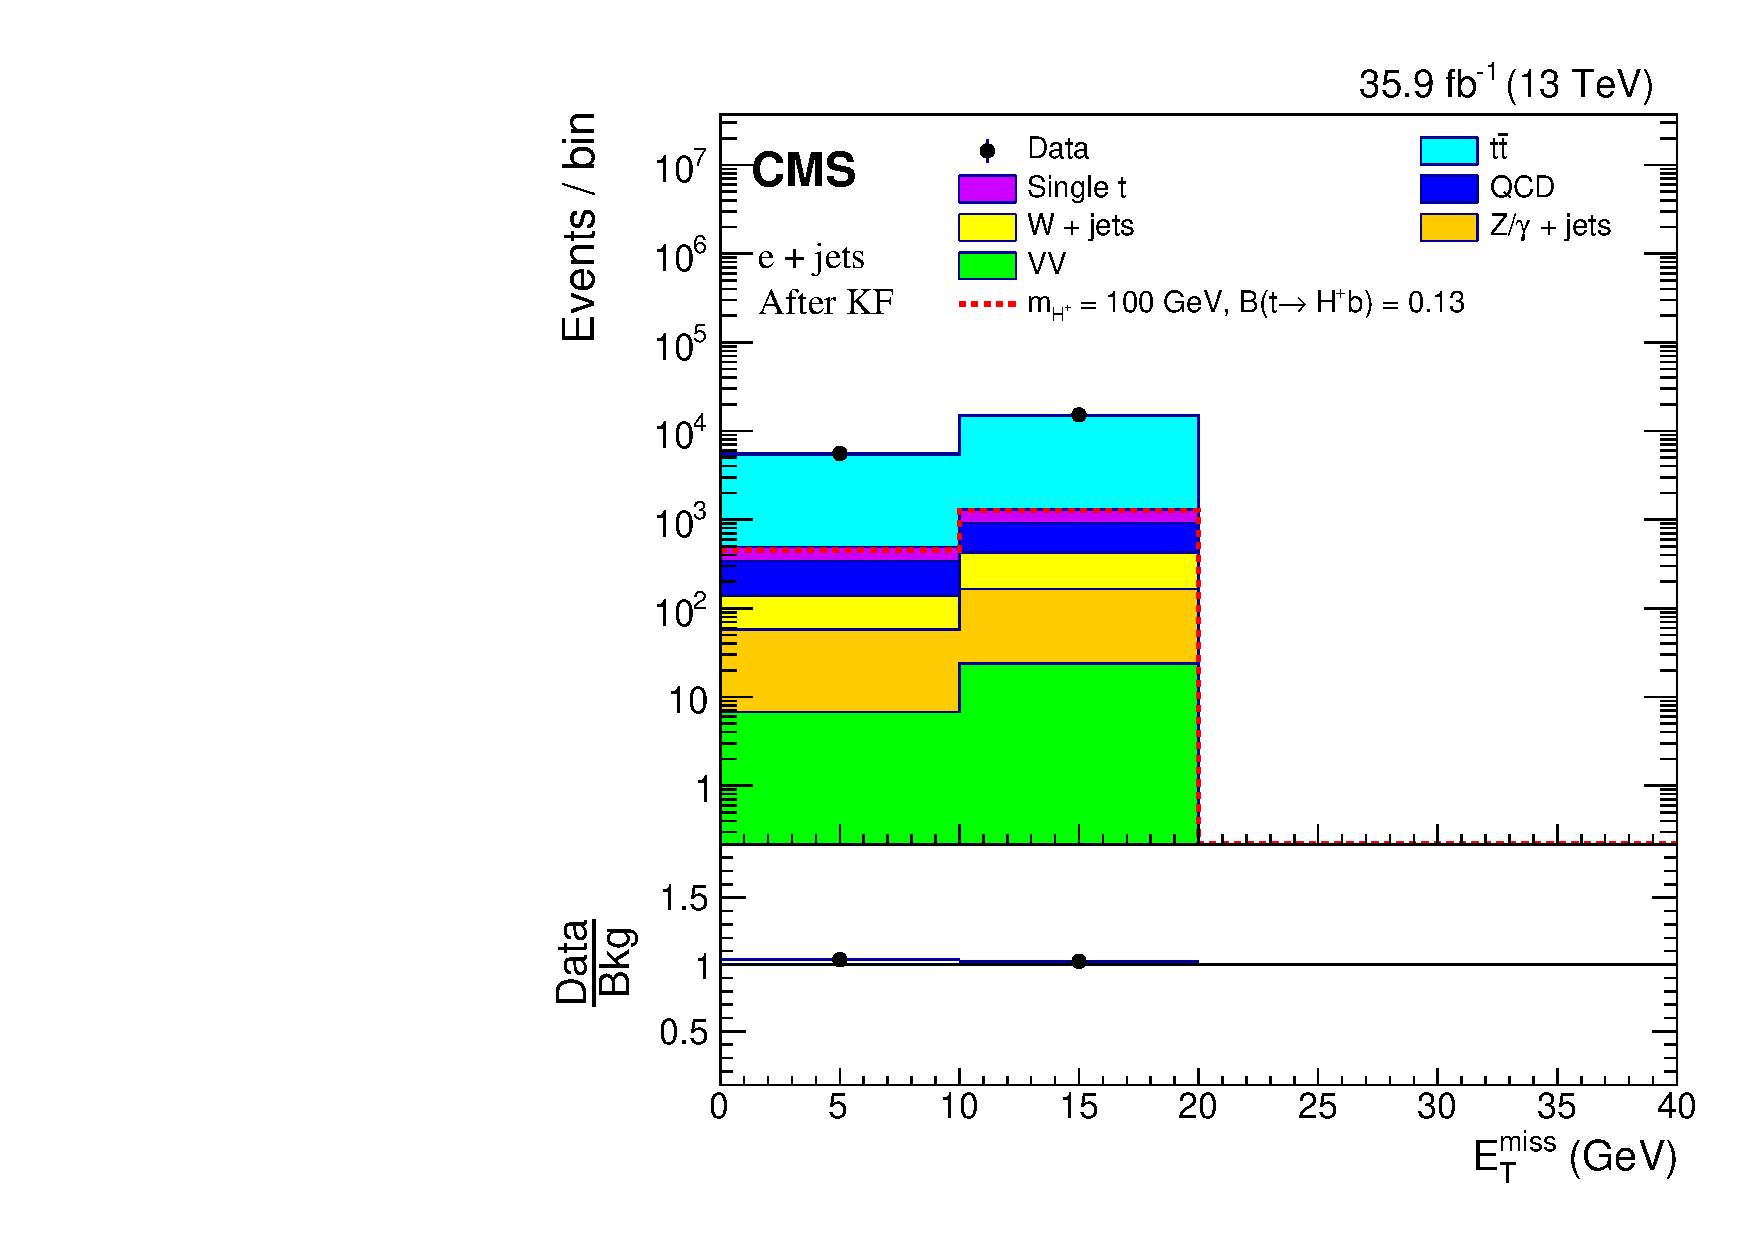
\includegraphics[width=0.45\linewidth]{Image/Electron/LowMET/KinFit/final_pt_met_eleKinFit.pdf}}
    \vfil
    \subfigure[Transverse mass of W-boson]{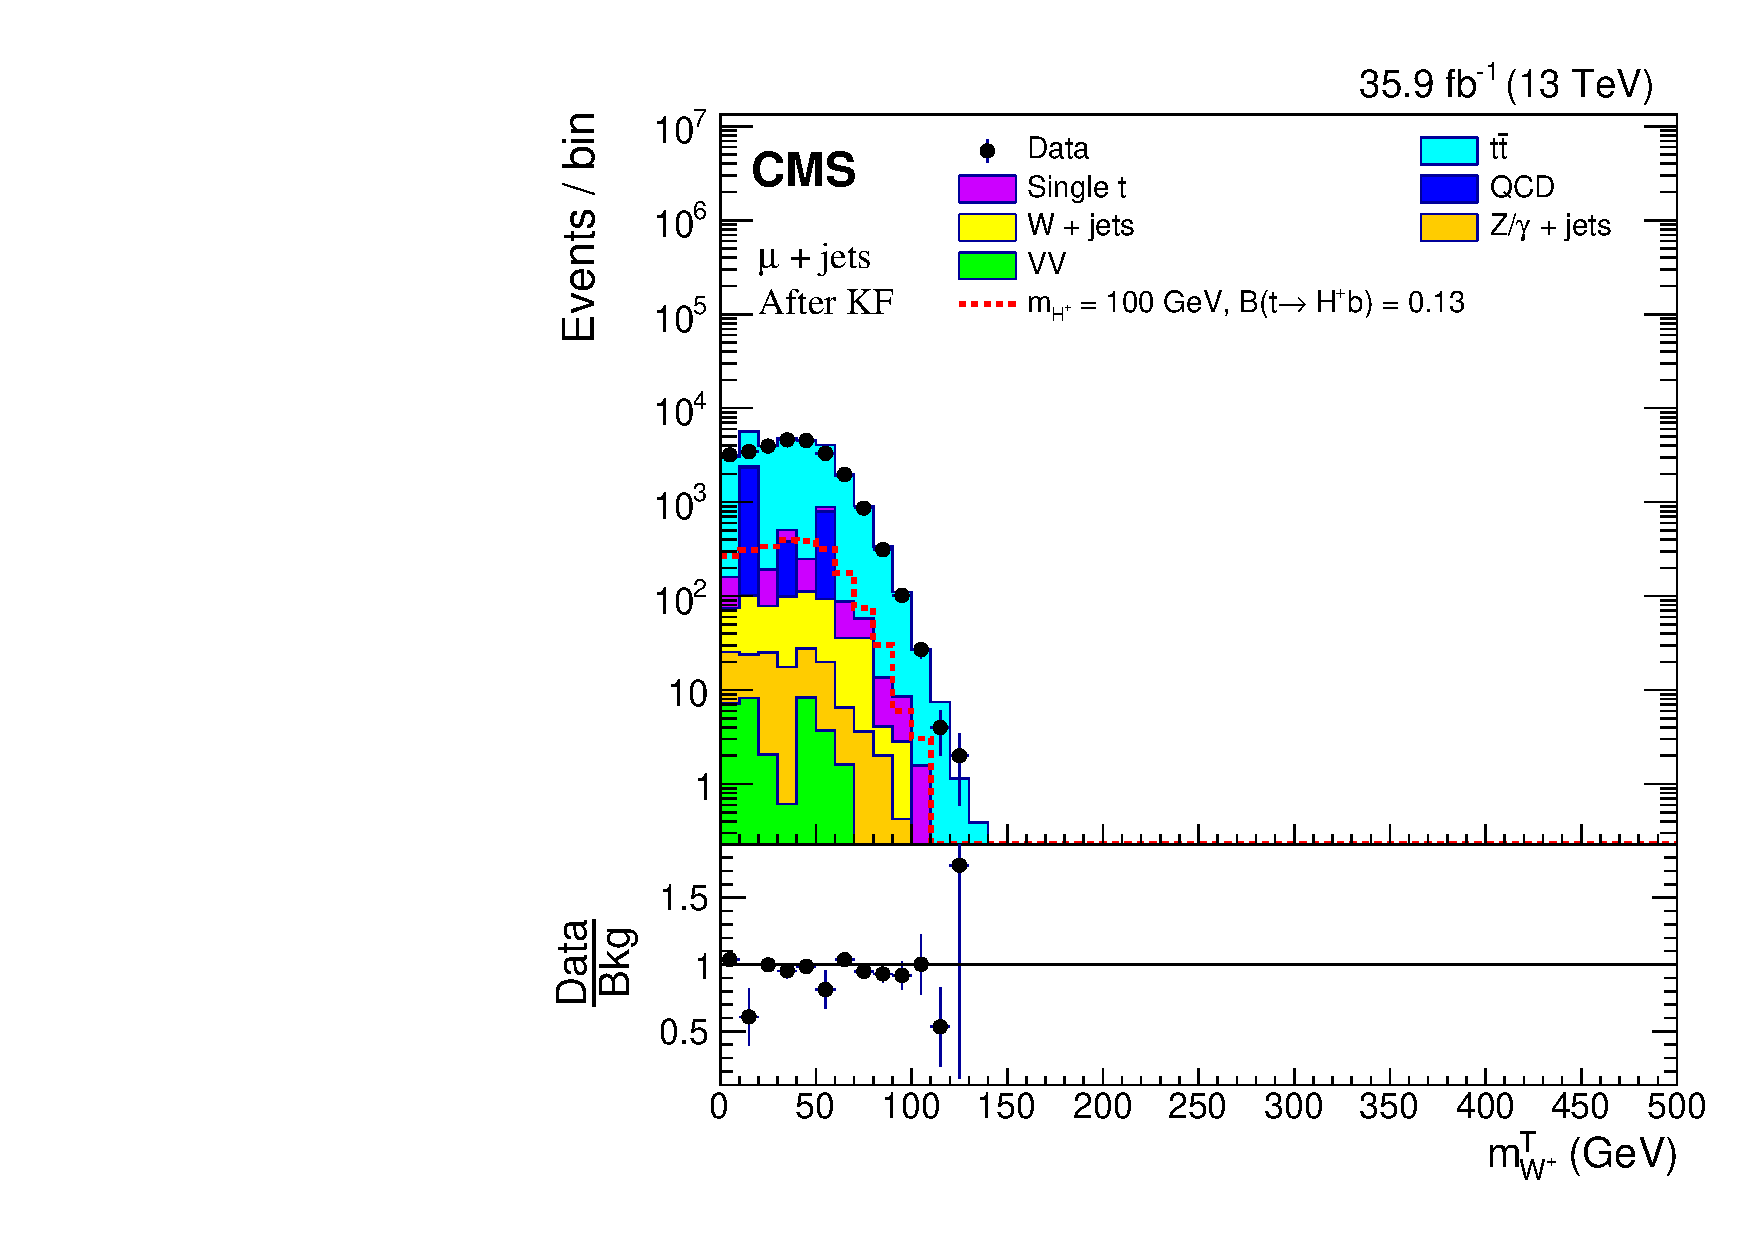
\includegraphics[width=0.45\linewidth]{Image/Muon/LowMET/KinFit/wmt_muKinFit.pdf}}
    \subfigure[Transverse mass of W-boson]{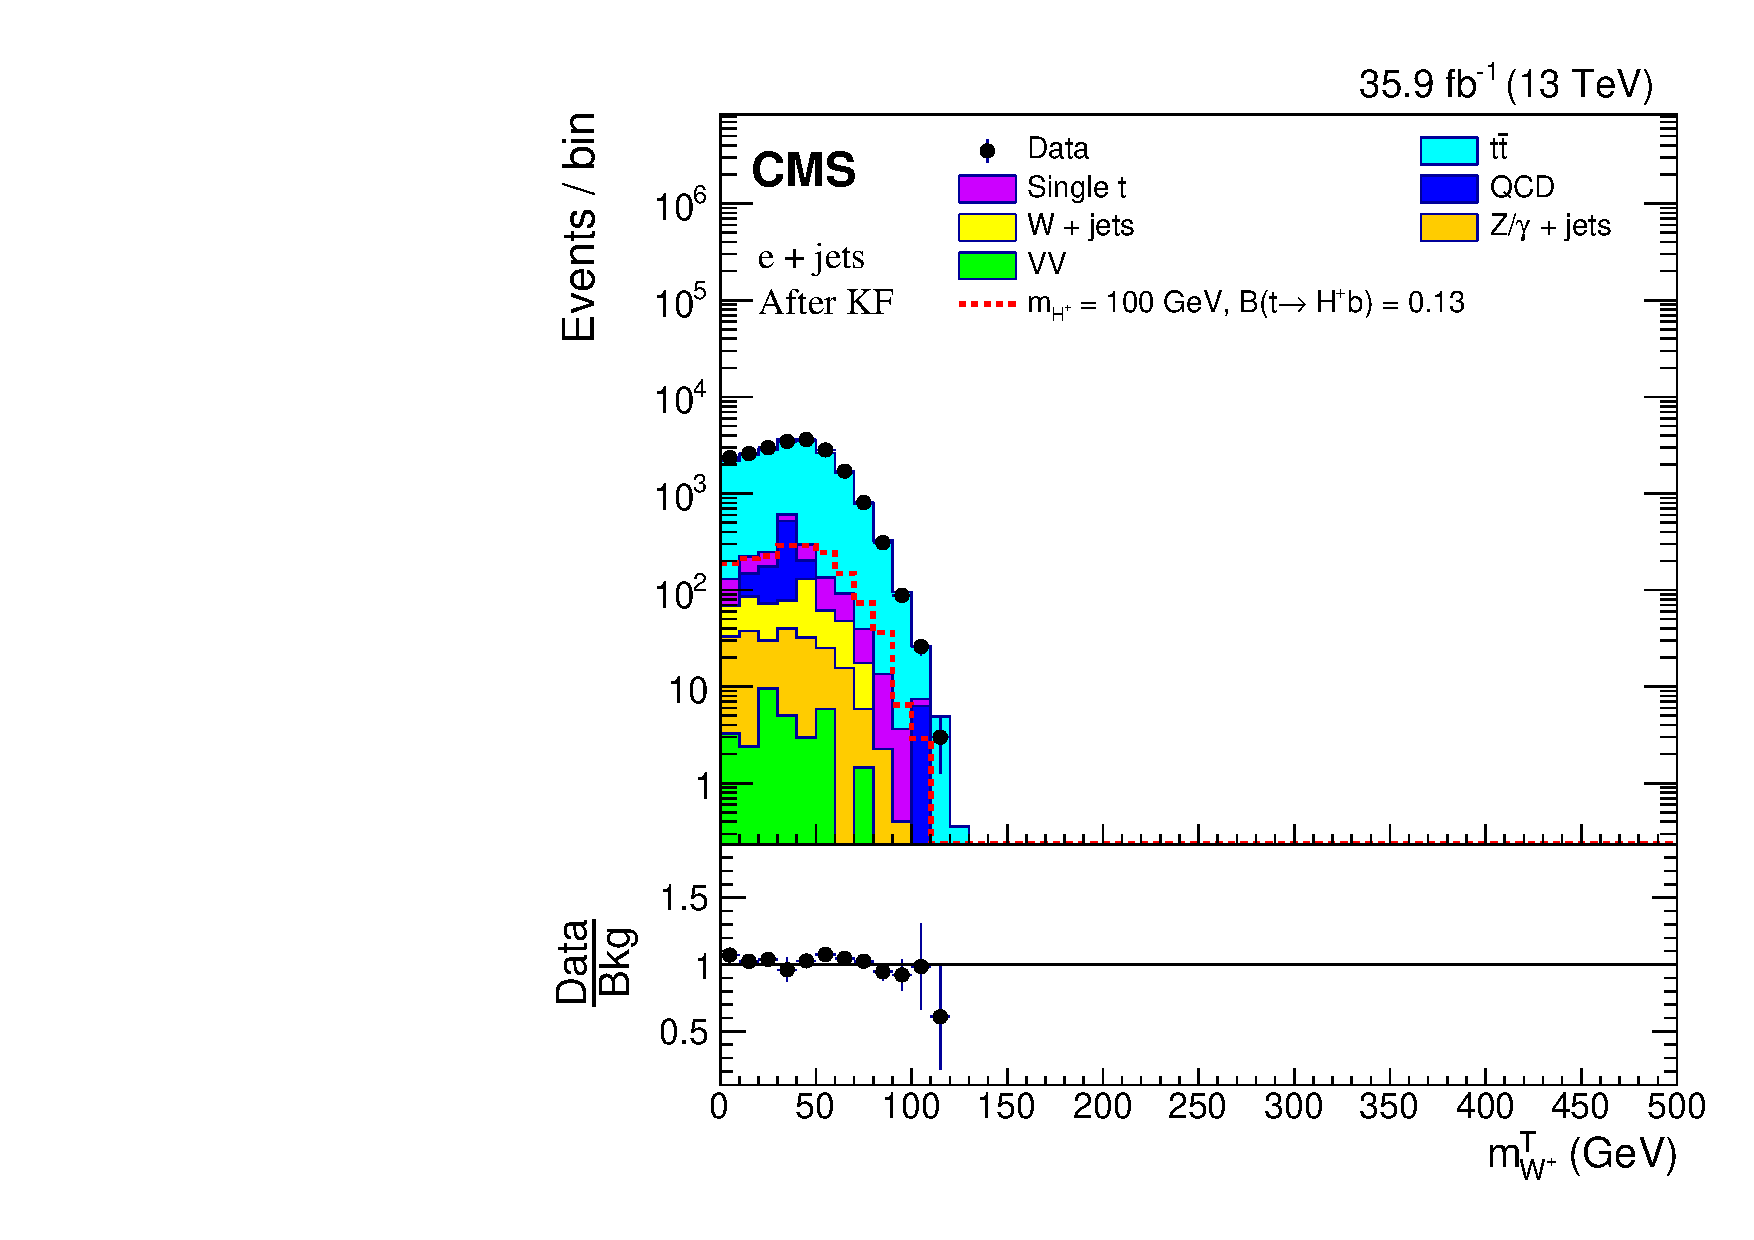
\includegraphics[width=0.45\linewidth]{Image/Electron/LowMET/KinFit/wmt_eleKinFit.pdf}}
    \caption{Control plots in $\MET <$ 20 GeV region, after kinematic fit selection as described
        in Sec.~\ref{s:secEvtSel}, for muons + jets and \ejets
    channel.}
    \label{fig:LowMET_kfitPlot3}
\end{figure}


    \begin{figure}
    \centering  
    \subfigure[\mjj without c-tagging. \label{subfig:mjj_LowMET_kfit_CTagIncL_muKinFit}]
    {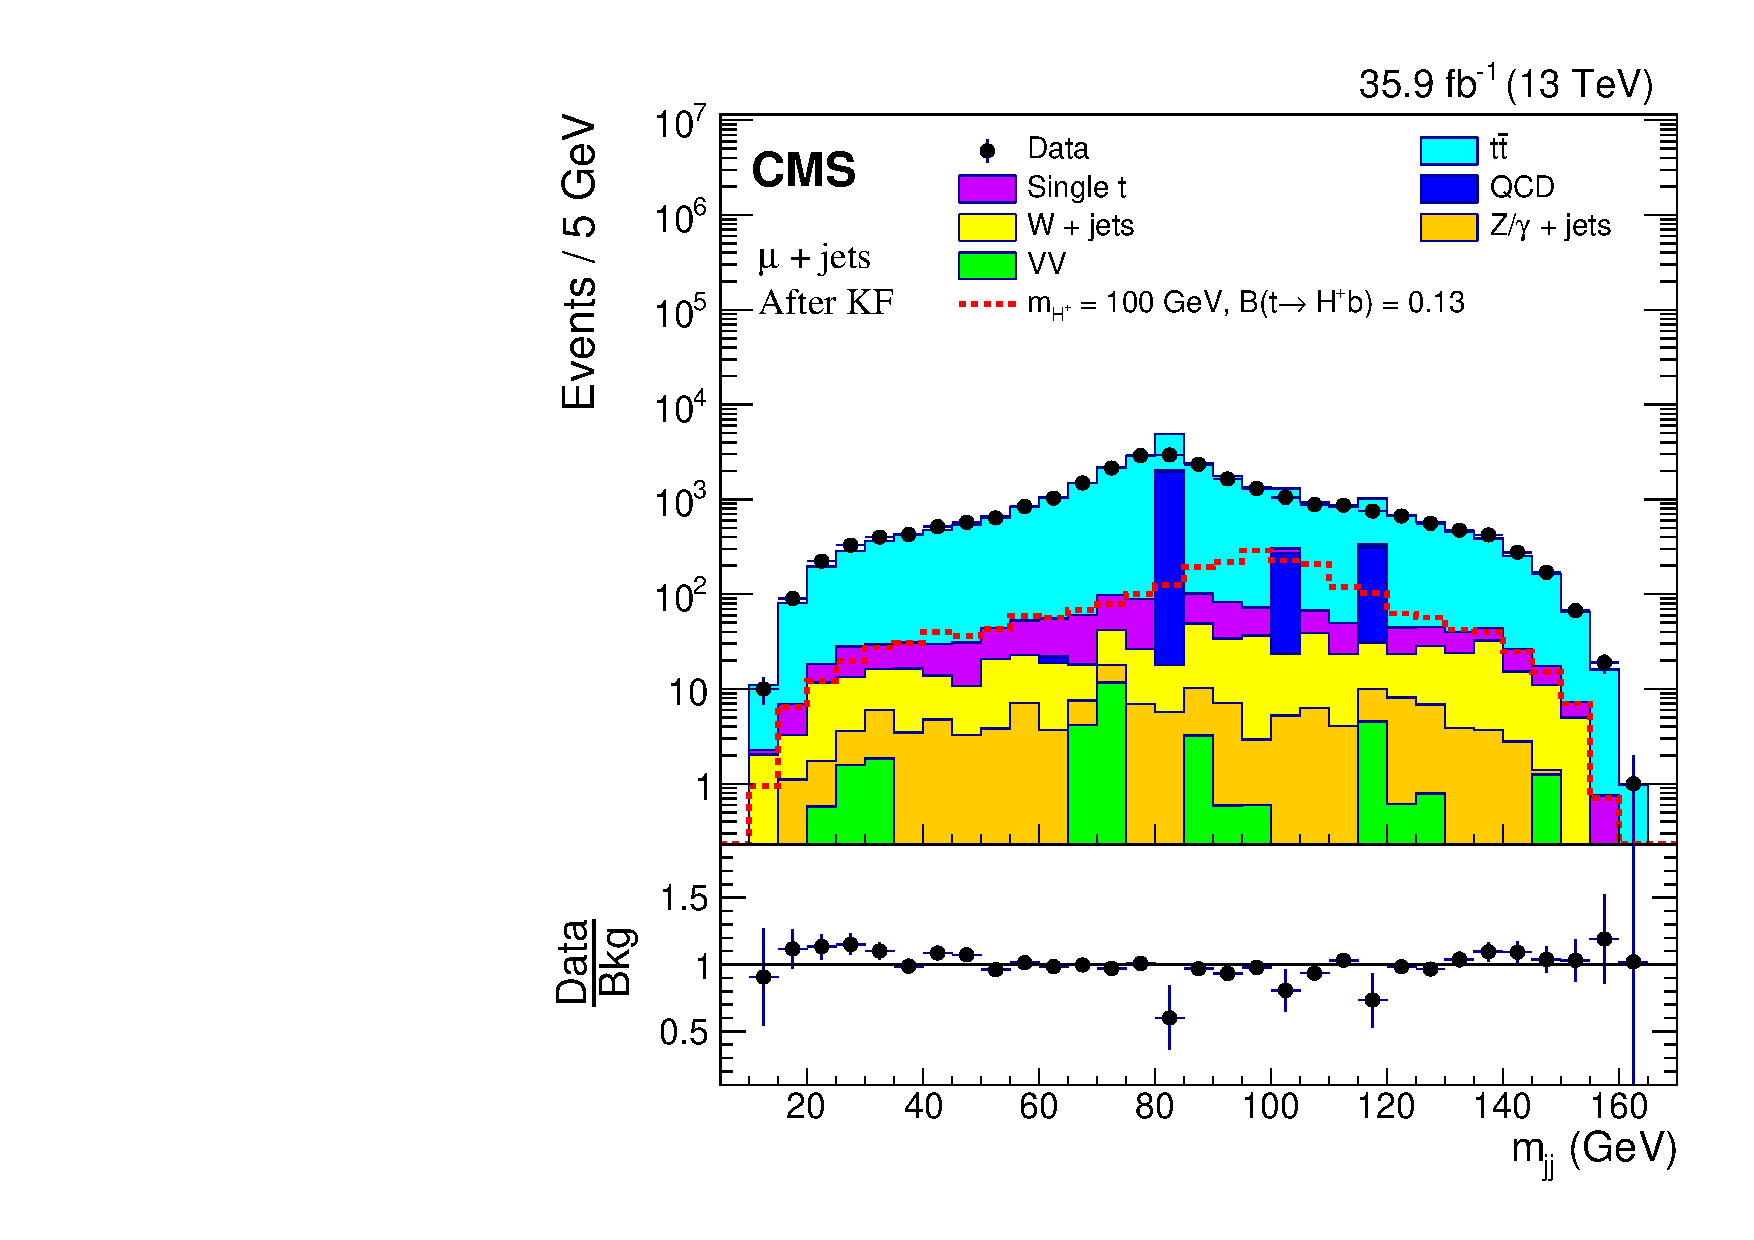
\includegraphics[width=0.50\linewidth]{Image/Muon/LowMET/KinFit/mjj_kfit_CTagIncL_muKinFit.pdf}}
    \subfigure[\mjj without c-tagging.\label{subfig:mjj_LowMET_kfit_CTagIncL_eleKinFit}]
    {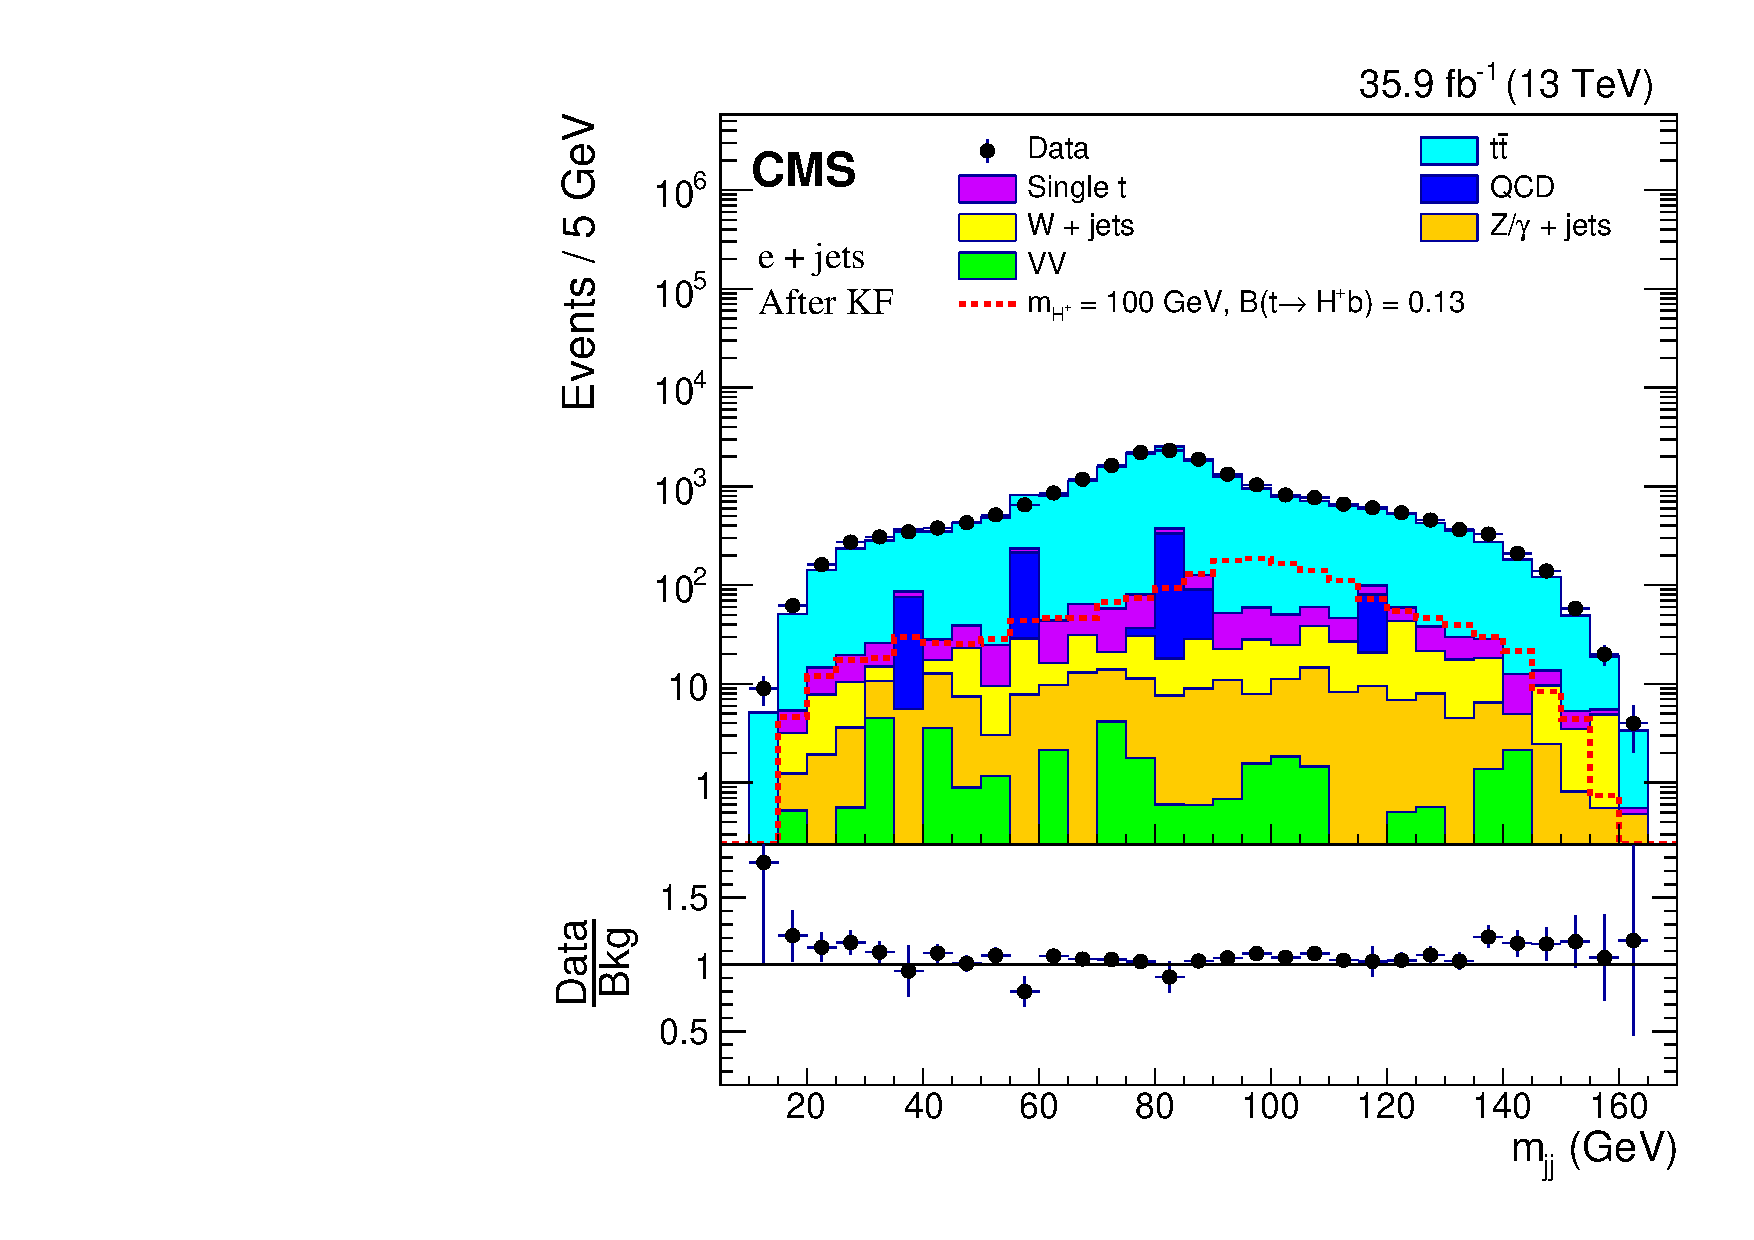
\includegraphics[width=0.50\linewidth]{Image/Electron/LowMET/KinFit/mjj_kfit_CTagIncL_eleKinFit.pdf}}
    \caption{Control plots in $\MET <$ 20 GeV region: distribution of \mjj from inclusive
        event category without charm-tagging for \mujets and \ejets channel.}
    \label{fig:LowMET_mjjInc}
    \end{figure}

    \begin{figure}
    \centering  
    \subfigure[\mjj for loose WP. \label{subfig:mjj_LowMET_kfit_muKinFit}]
    {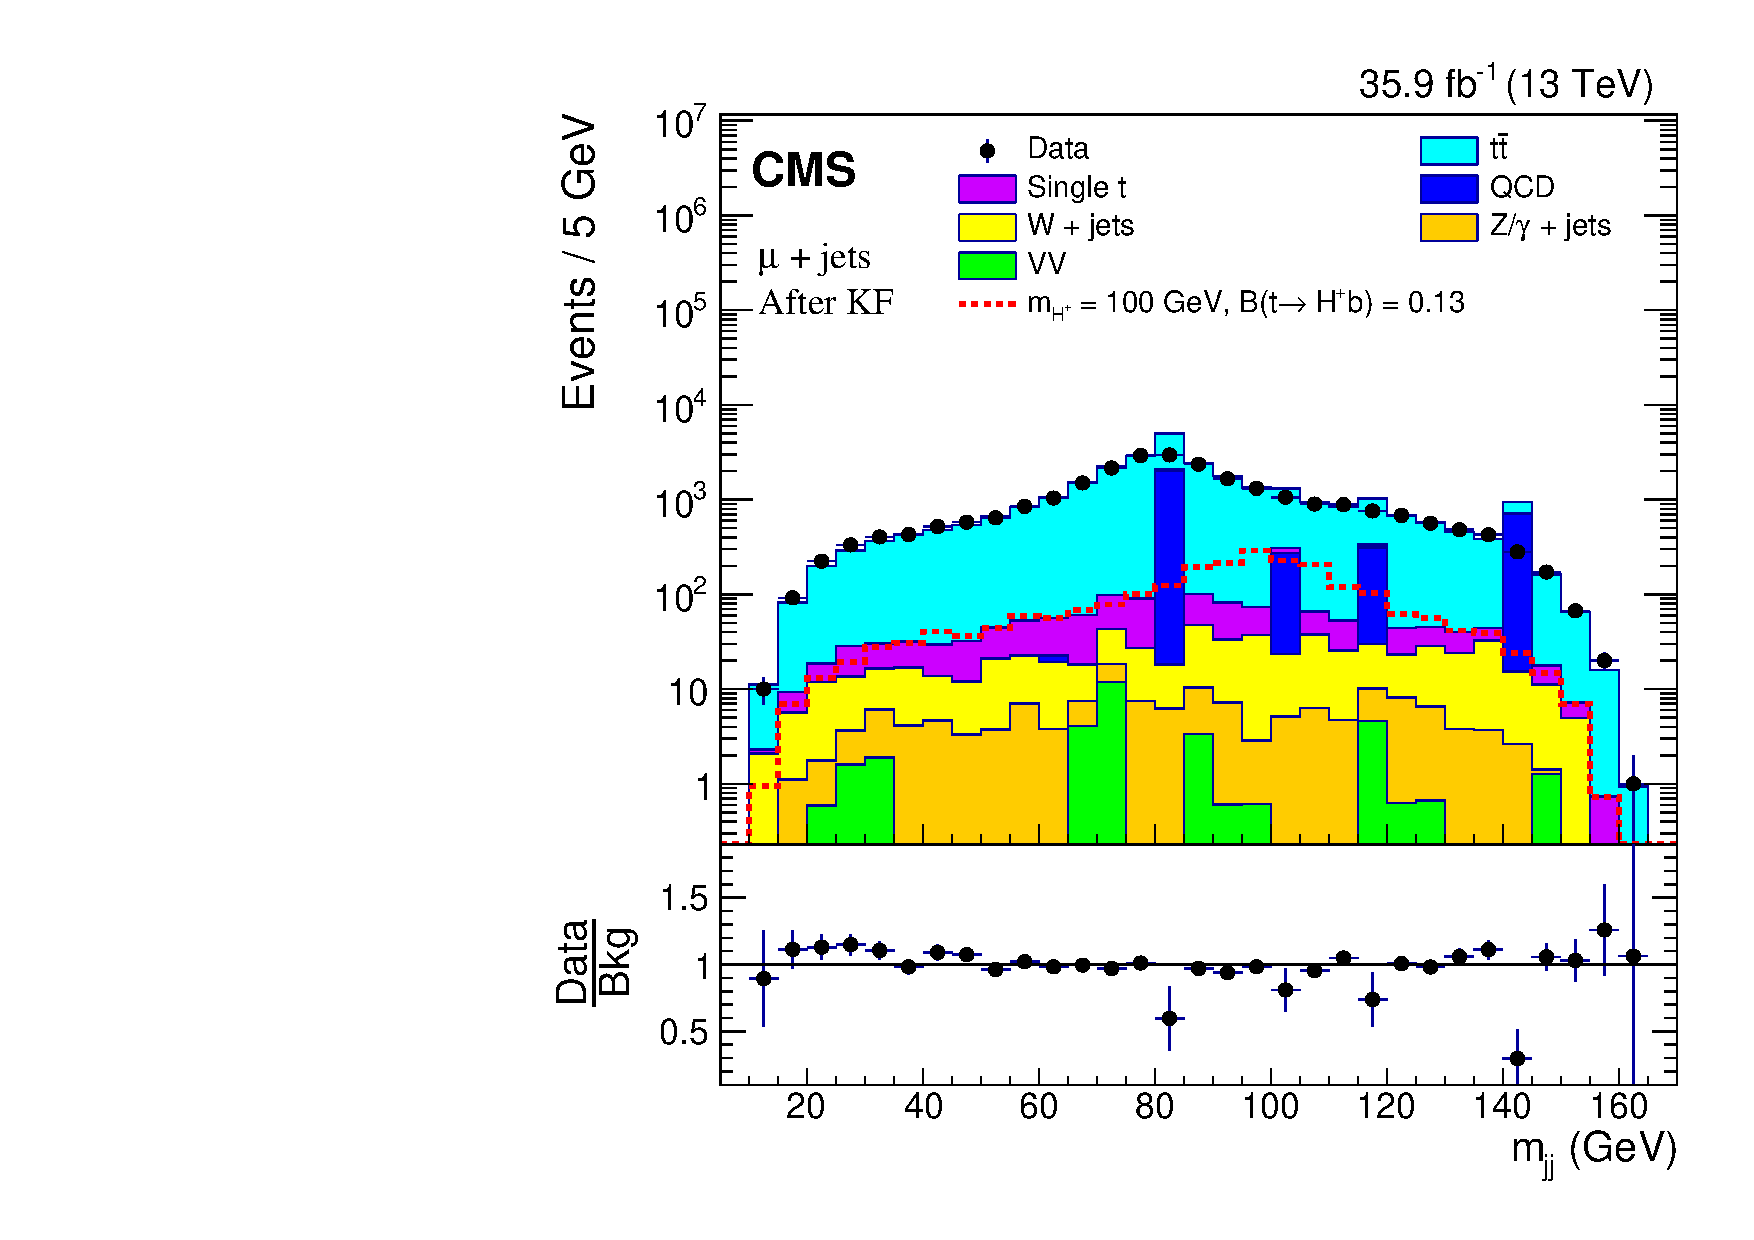
\includegraphics[width=0.50\linewidth]{Image/Muon/LowMET/KinFit/mjj_kfit_muKinFit.pdf}}
    \subfigure[\mjj for loose WP.\label{subfig:mjj_LowMET_kfit_eleKinFit}]
    {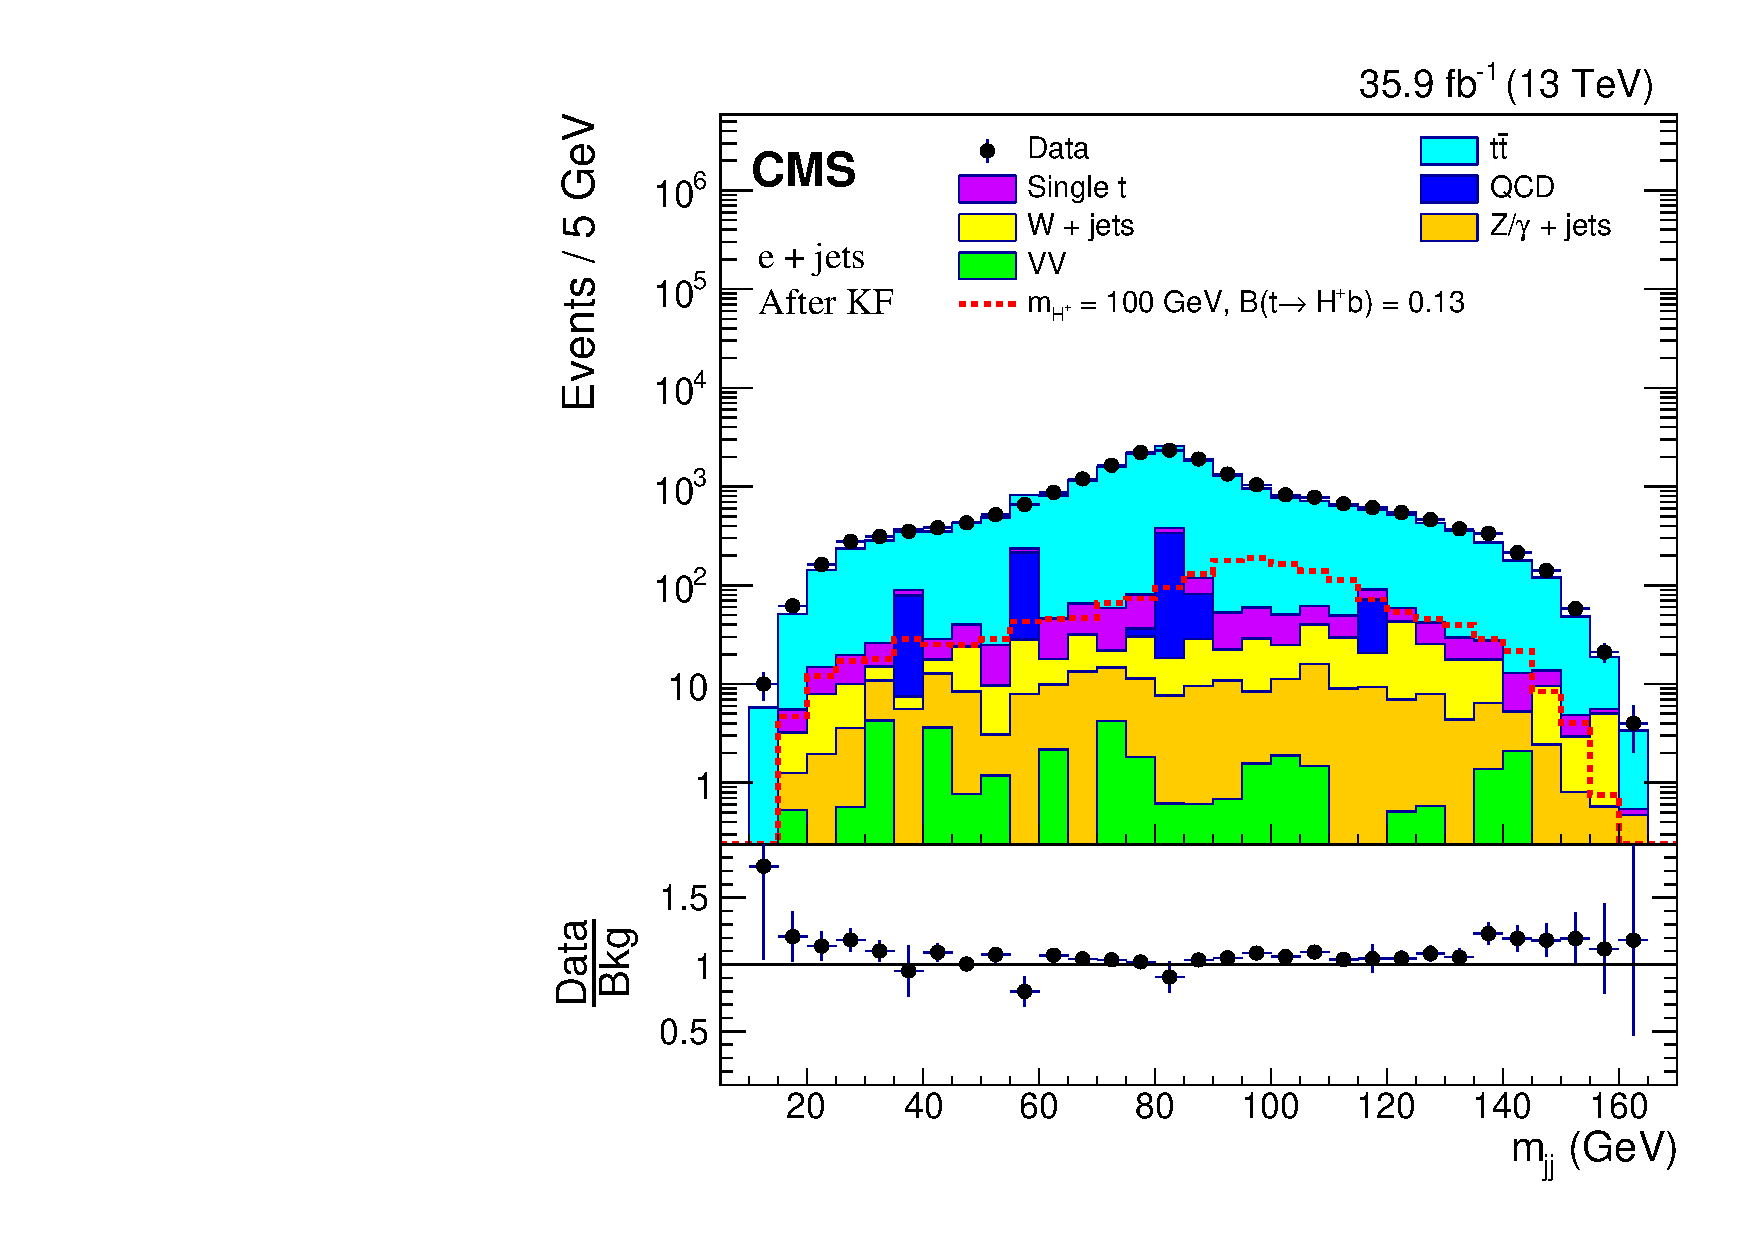
\includegraphics[width=0.50\linewidth]{Image/Electron/LowMET/KinFit/mjj_kfit_eleKinFit.pdf}}
    \caption{Control plots in $\MET <$ 20 GeV region: distribution of \mjj for loose inclusive charm 
        working point for \mujets and \ejets channel.}
    \label{fig:LowMET_mjjCTagL}
    \end{figure}

    \begin{figure}
    \centering  
    \subfigure[Mjj in loose category for muon channel]
    {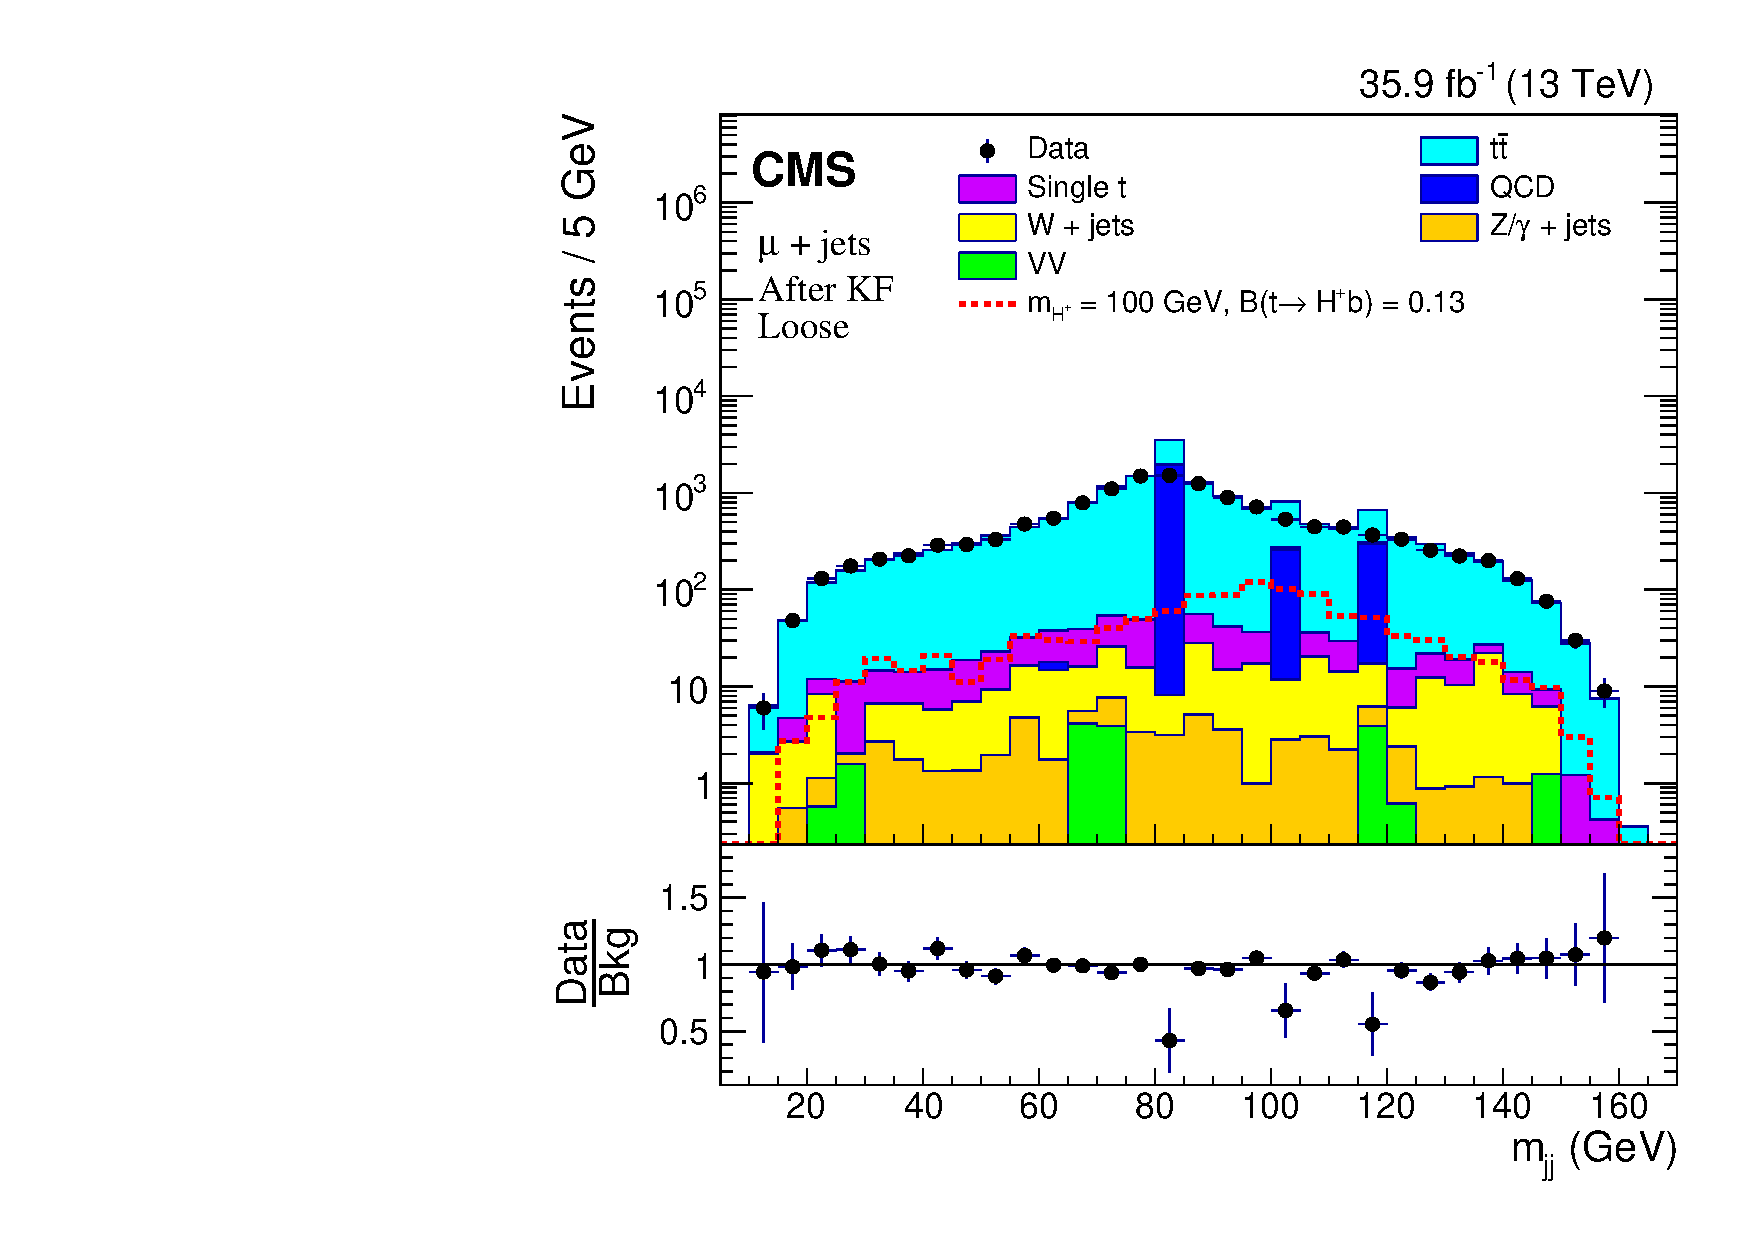
\includegraphics[width=0.45\linewidth]{Image/Muon/LowMET/KinFit/mjj_kfit_CTagExL_muKinFit.pdf}}
    \subfigure[Mjj in loose category for electron channel]
    {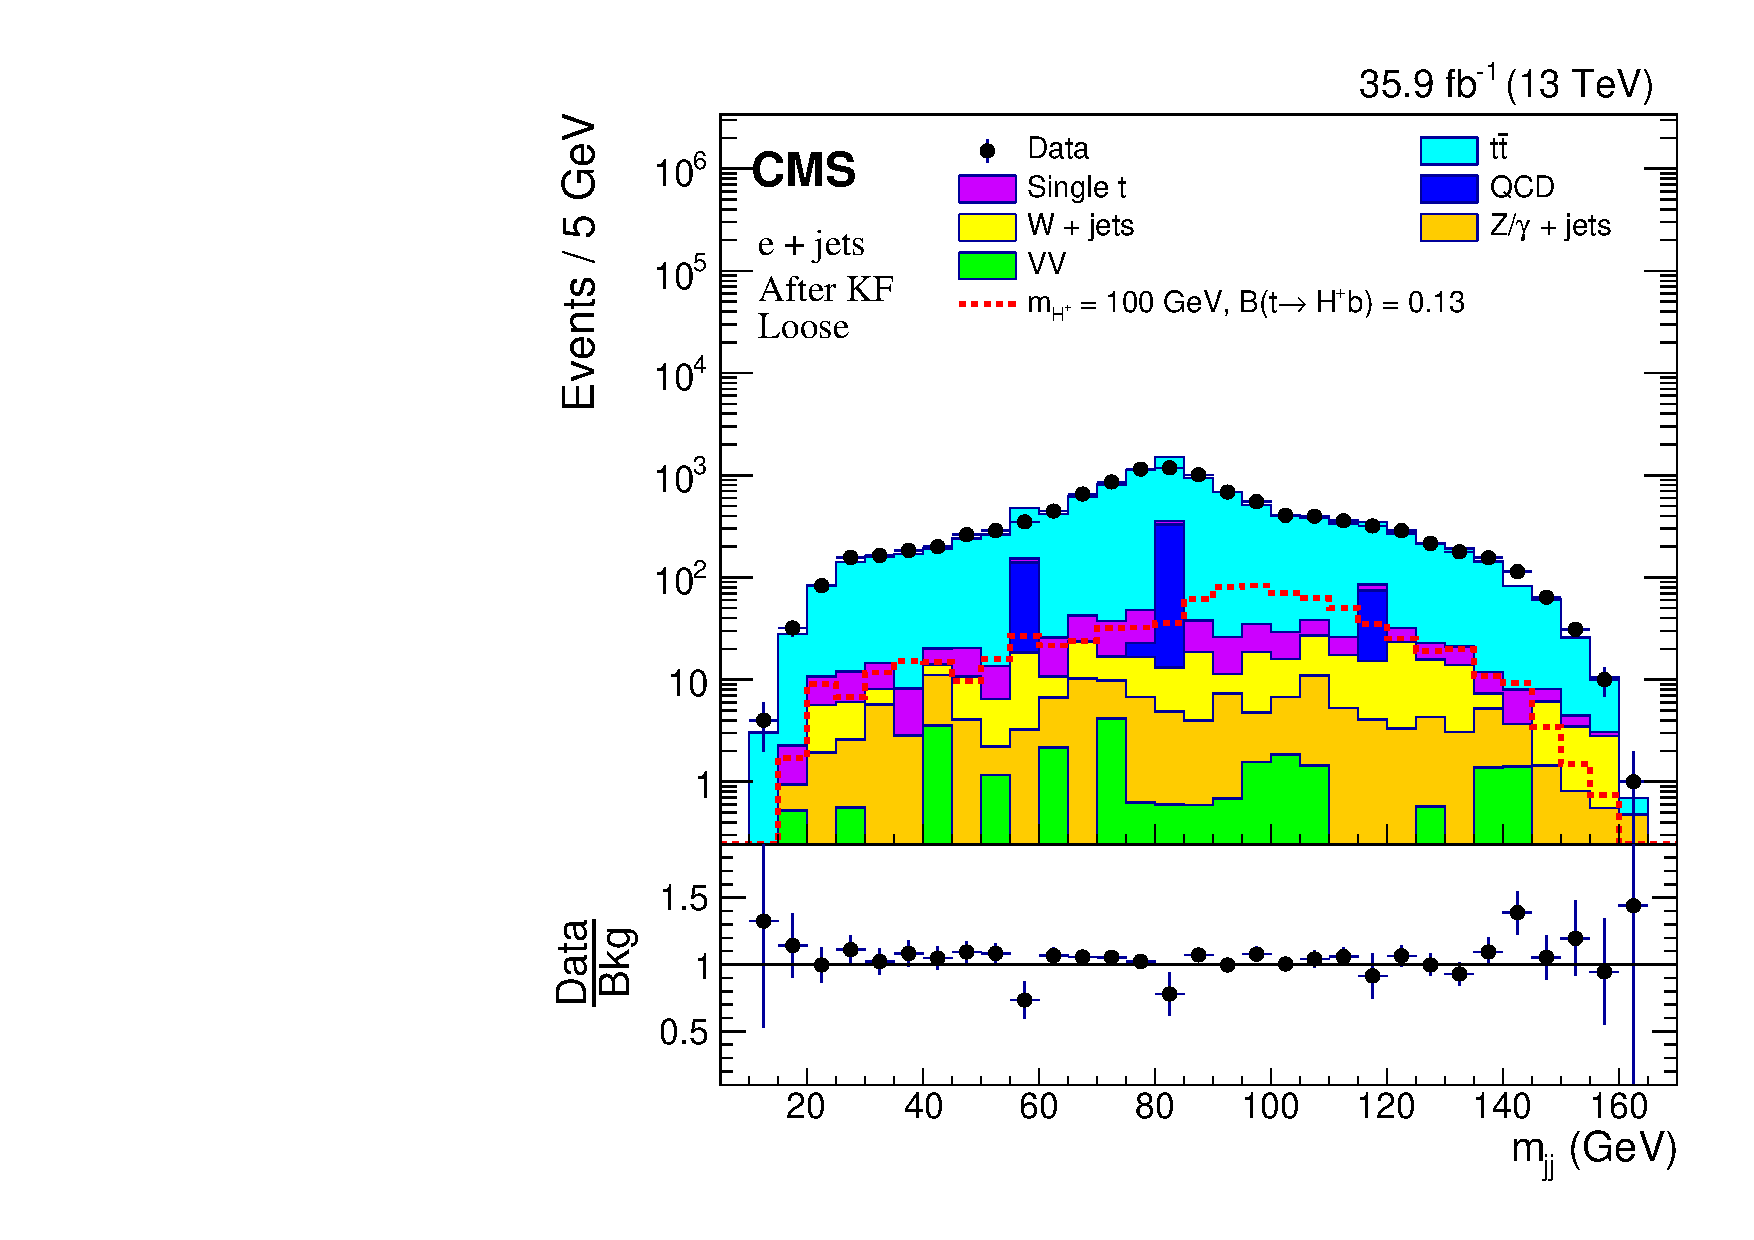
\includegraphics[width=0.45\linewidth]{Image/Electron/LowMET/KinFit/mjj_kfit_CTagExL_eleKinFit.pdf}}
    \vfil
    \subfigure[Mjj in medium category for muon channel]
    {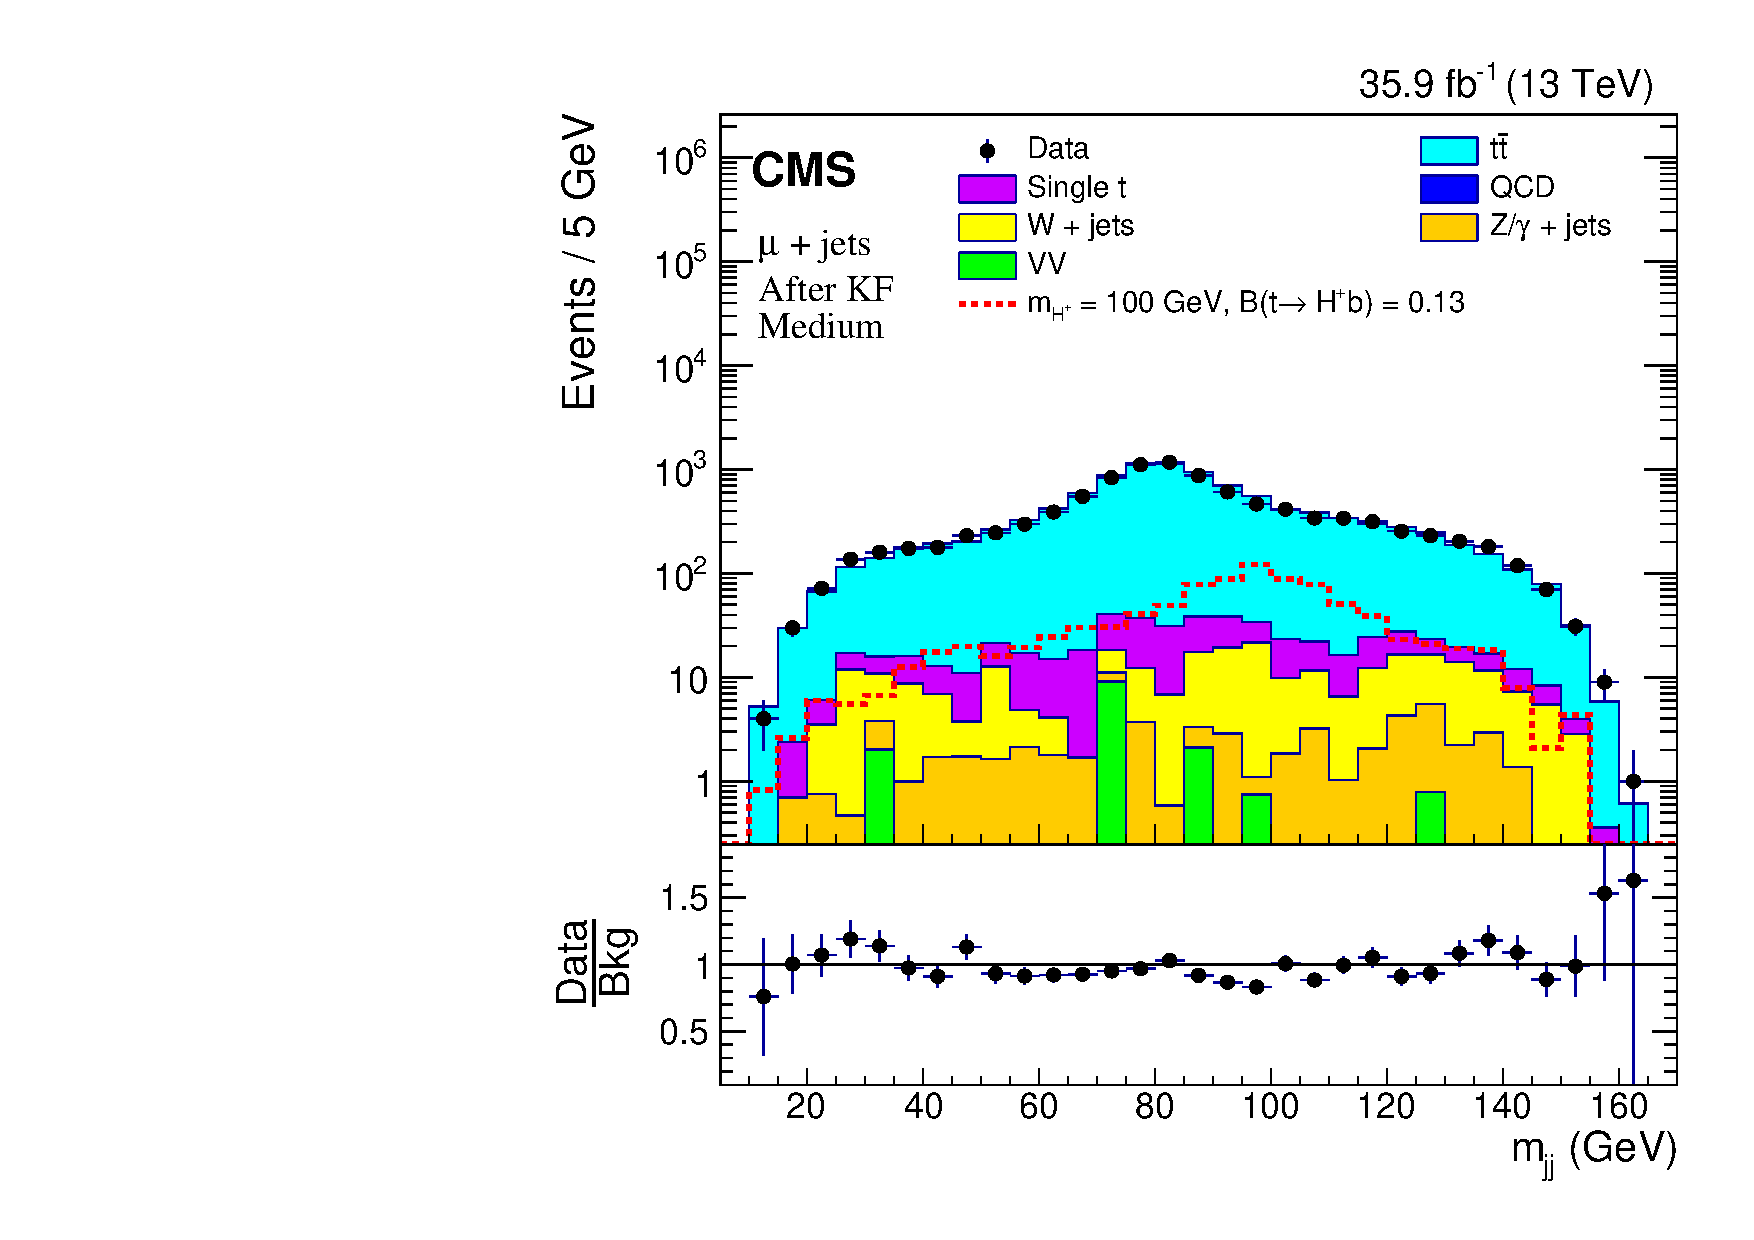
\includegraphics[width=0.45\linewidth]{Image/Muon/LowMET/KinFit/mjj_kfit_CTagExM_muKinFit.pdf}}
    \subfigure[Mjj in medium category for electron channel]
    {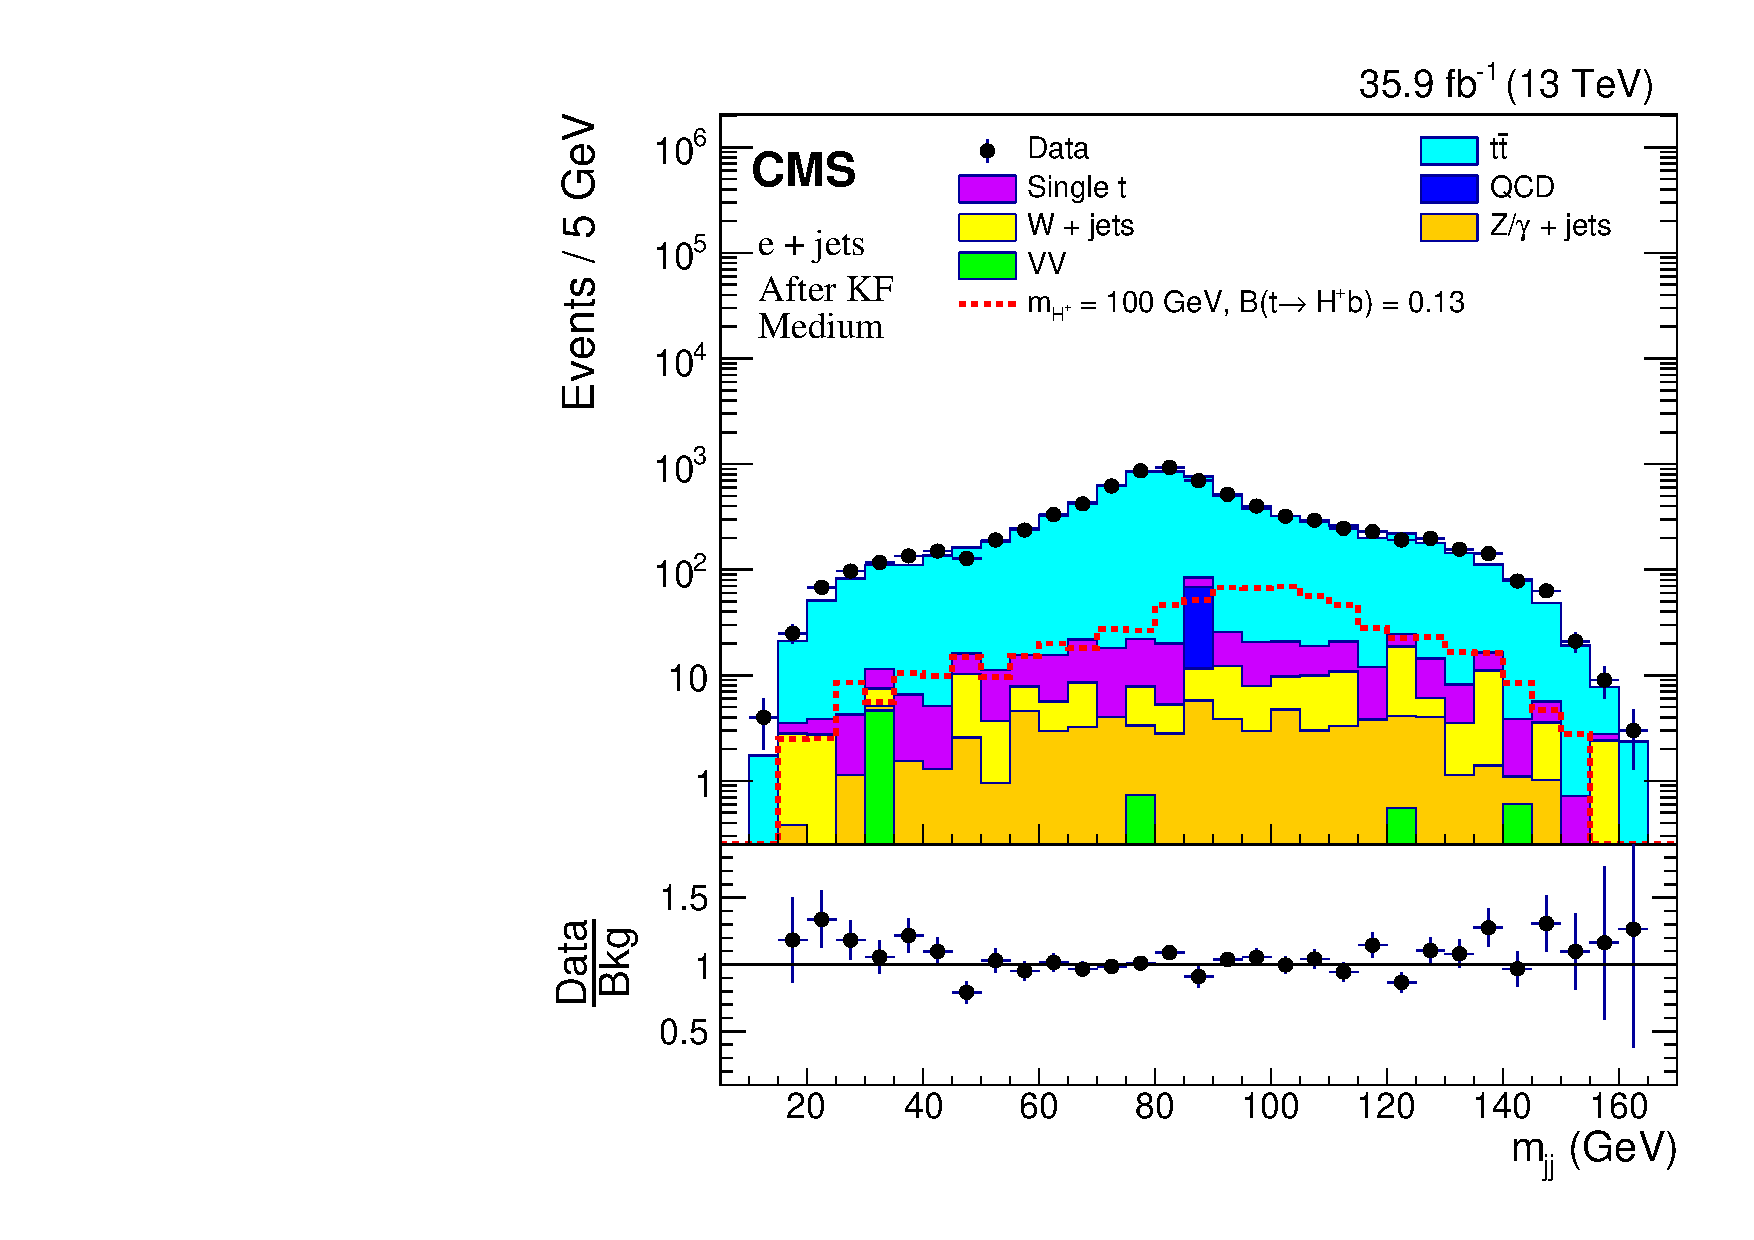
\includegraphics[width=0.45\linewidth]{Image/Electron/LowMET/KinFit/mjj_kfit_CTagExM_eleKinFit.pdf}}
    \vfil
    \subfigure[Mjj in tight category for muon channel]
    {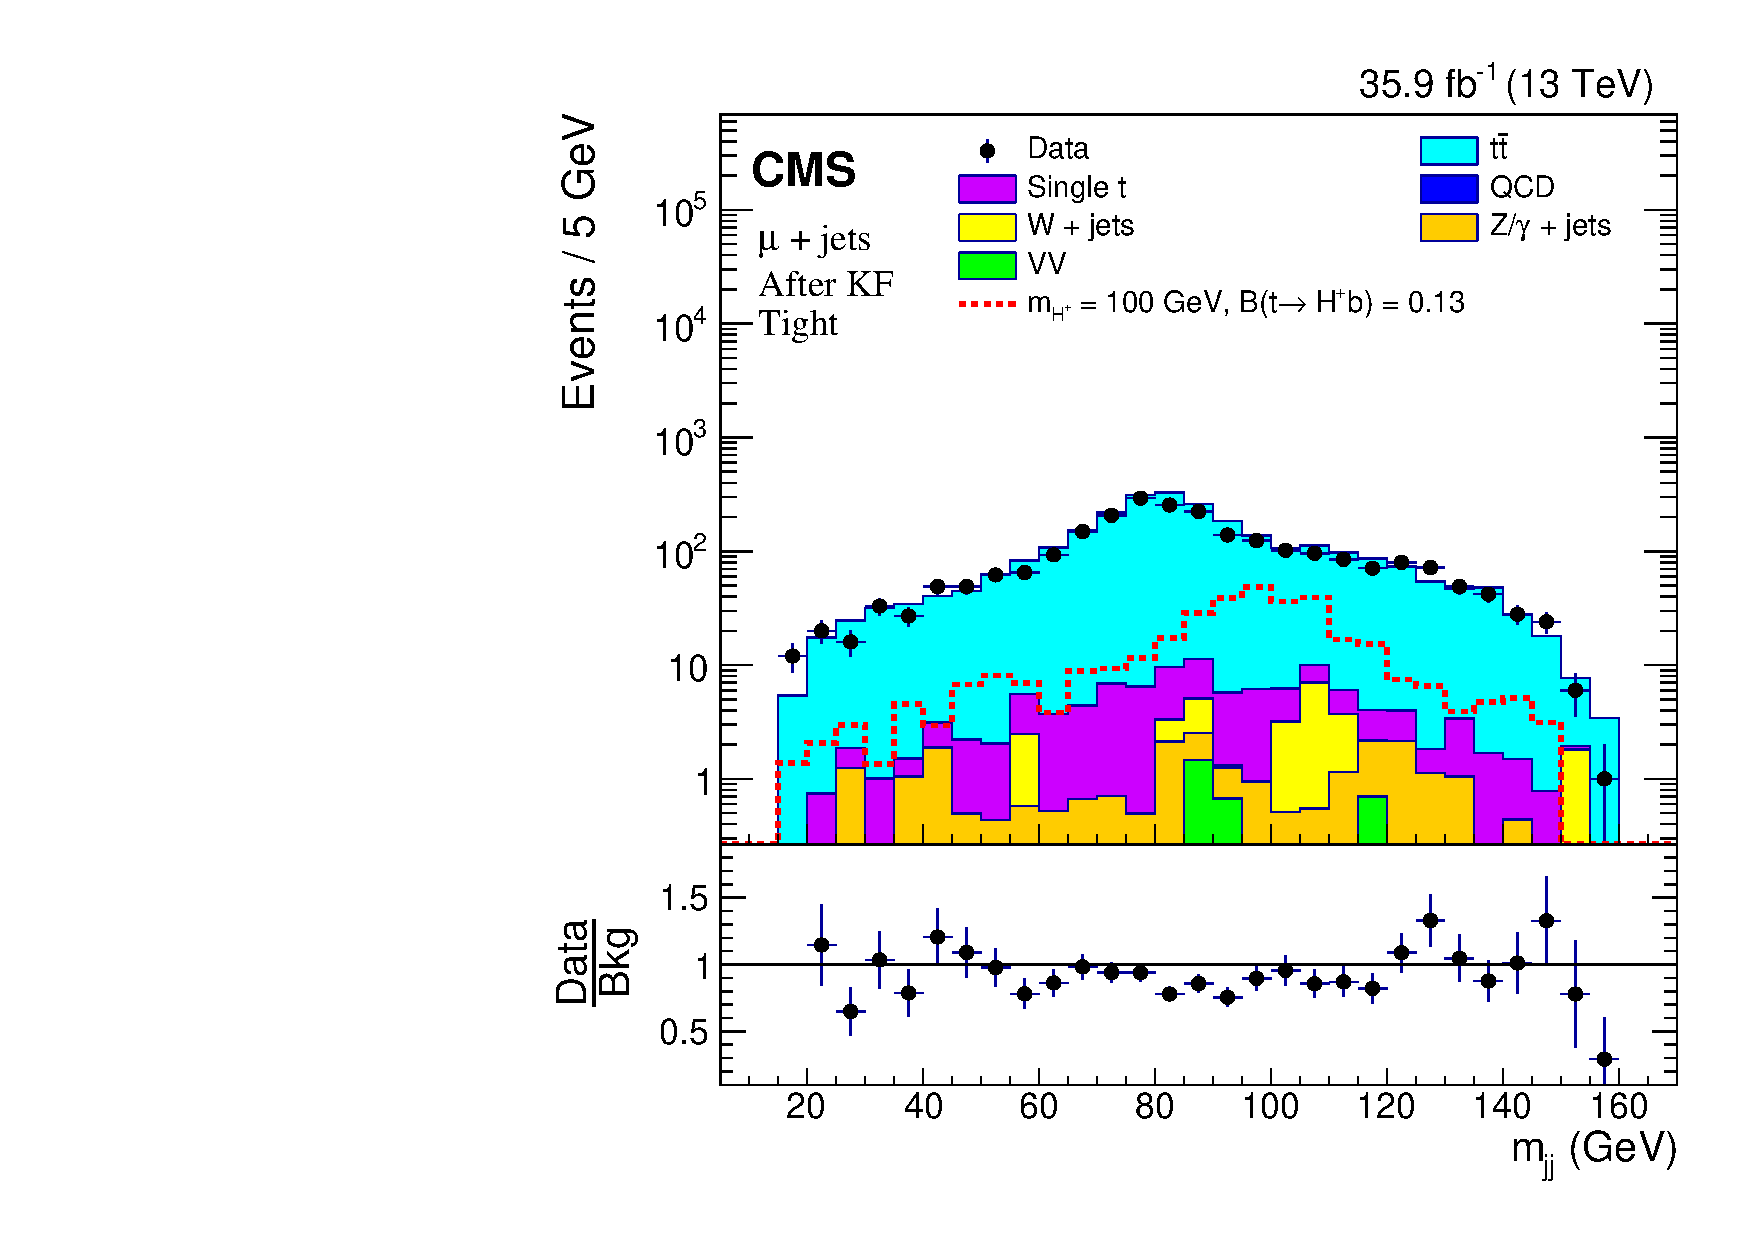
\includegraphics[width=0.45\linewidth]{Image/Muon/LowMET/KinFit/mjj_kfit_CTagExT_muKinFit.pdf}}
    \subfigure[Mjj in tight category for electron channel]
    {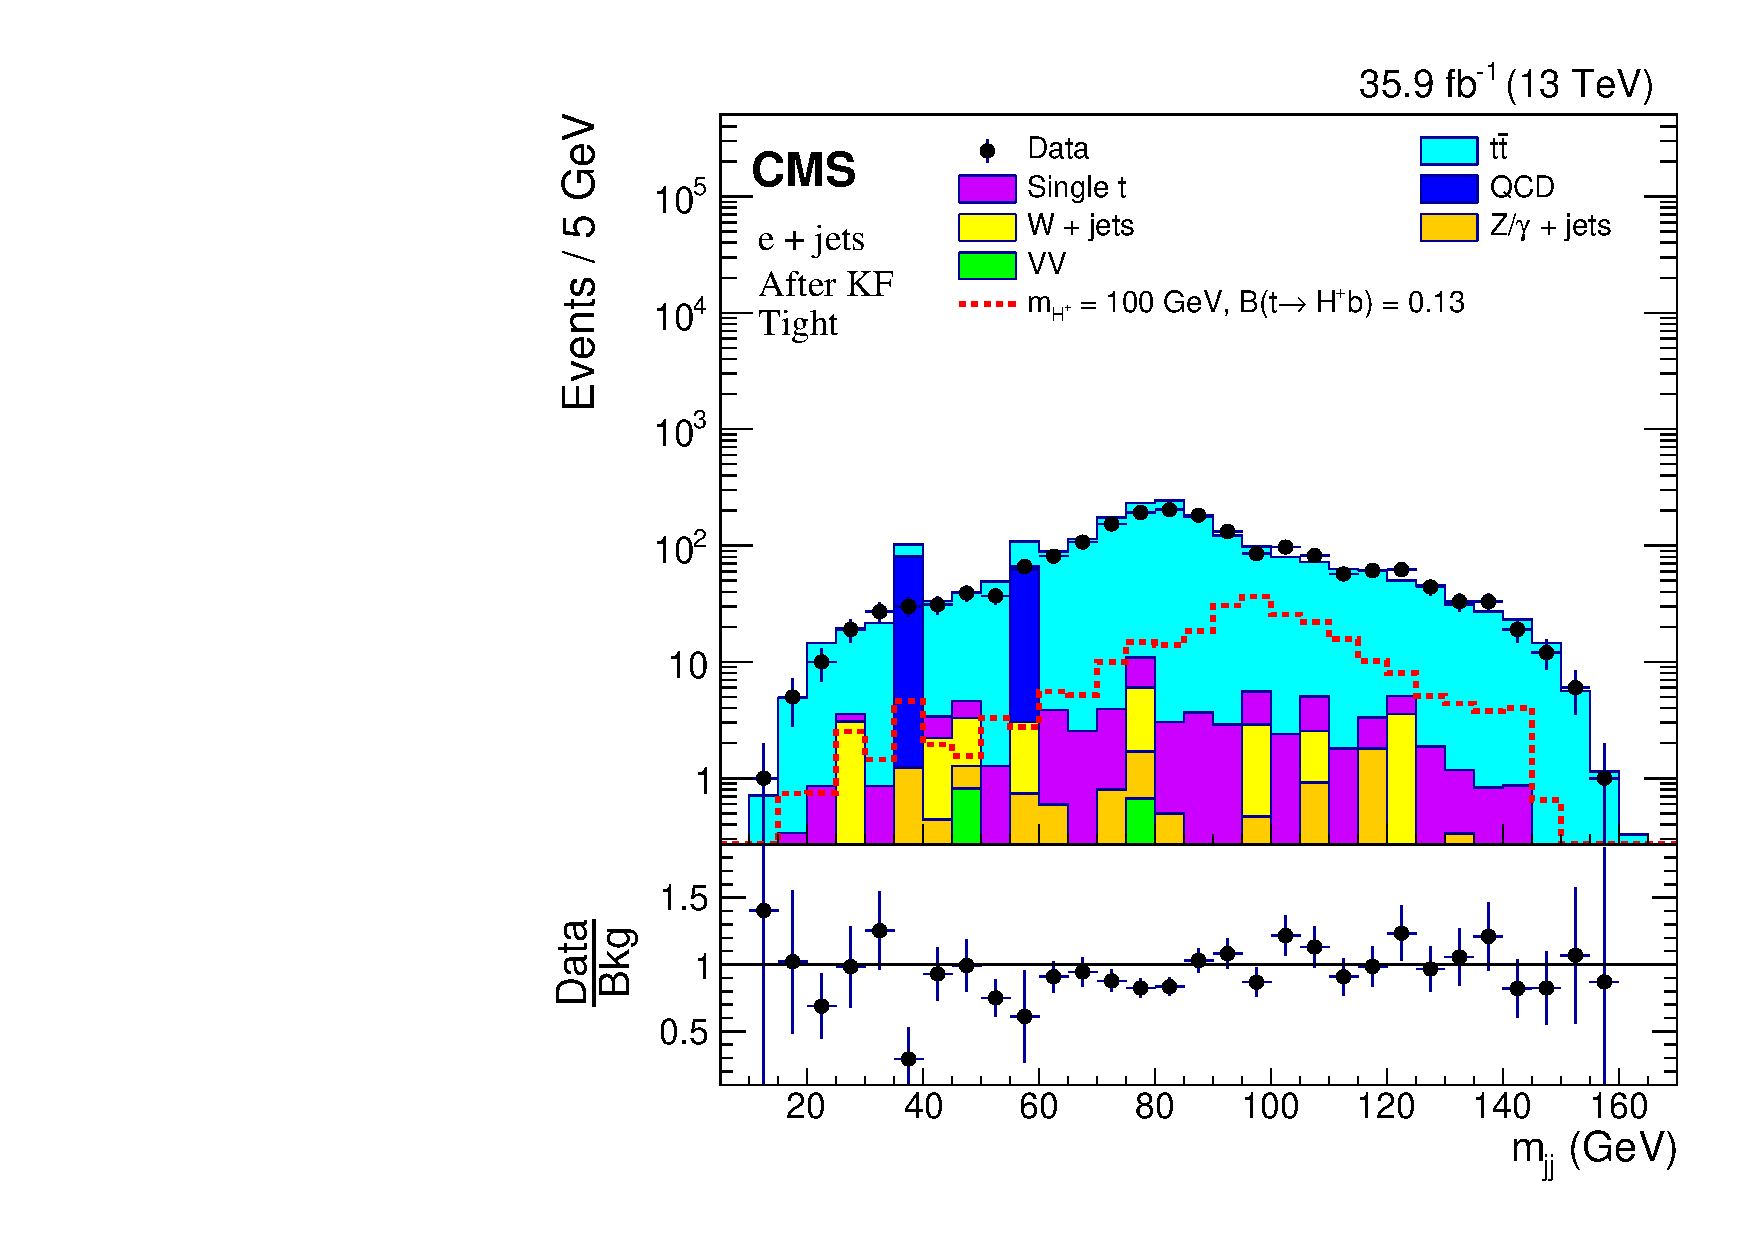
\includegraphics[width=0.45\linewidth]{Image/Electron/LowMET/KinFit/mjj_kfit_CTagExT_eleKinFit.pdf}}
    \caption{Control plots in $\MET <$ 20 GeV region: distribution of \mjj from exclusive charm categories as described in
    Sec.~\ref{ss:mjj_cTagEx} for \mujets and \ejets channel. The signal significance is different across different
    exclusive categories.}
    \label{fig:LowMET_mjjCTagEx}
    \end{figure}

